\begin{longtable}{p{0.03\textwidth} | p{0.22\textwidth} | p{0.22\textwidth} | p{0.22\textwidth} | p{0.22\textwidth}}
\hline
\textbf{id} & \textbf{Hugtök} & \textbf{Skilgreining} & \textbf{Skýring} & \textbf{Athugasemdir} \\
\hline
0 & \hypertarget{row:0}{MISSING} & ... &  &  \\
\hline
6 & \hypertarget{row:6}{\(n\)-und, \(n\)-d, röðuð \(n\)-und, röðuð \hbox{\(n\)-d}} & $n$-\textit{und}, þar sem $n$ er \hyperlink{row:3475}{náttúruleg tala}, samanstendur af $n$ \hyperlink{row:2123}{hlutum} í tiltekinni röð. $n$-undin sem inniheldur hlutina $a_1, \ldots, a_n$ í þessari röð er táknuð með $(a_1, \ldots, a_n)$ & Ef $\{ A_i \}_{i=1}^n$ er \hyperlink{row:1229}{fjölskylda} af \hyperlink{row:3270}{mengjum} og $a_i \in A_i$ fyrir $i=1,\dots,n$ þá er $n$-undin $(a_1,\dots,a_n)$ \hyperlink{row:5128}{stak} í \hyperlink{row:3279}{faldmenginu} $\prod_{i=1}^n A_i$ &  \\
\hline
46 & \hypertarget{row:46}{aðgerð, reikniaðgerð} & \hyperlink{row:3282}{Vörpun} af gerðinni $X \times \cdots \times X \to X$ þar sem $X$ er \hyperlink{row:3270}{mengi} kallast \textit{reikniaðgerð} á $X$ &  & Koma með dæmi? \\
\hline
65 & \hypertarget{row:65}{aðlæg hlið} & Tvær \hyperlink{row:2048}{hliðar} \hyperlink{row:3161}{marghyrnings} sem \hyperlink{row:4771}{skerast} í nákvæmlega einum \hyperlink{row:4001}{punkti} (í tveim \hyperlink{row:6087}{víddum}) eða tvær \hyperlink{row:1325}{hliðar} \hyperlink{row:3133}{margflötungs} sem skerast í einum eða fleiri punktum sem liggja allir á sömu \hyperlink{row:2911}{línu} (í þrem víddum) kallast \textit{aðlægar hliðar} &  & Koma með mynddæmi? \\
\hline
74 & \hypertarget{row:74}{aðmengi, ítak, bakmengi} & Sjá \hyperlink{row:3282}{vörpun} &  &  \\
\hline
234 & \hypertarget{row:234}{almennt brot} & \hyperlink{row:2072}{Hlutfall} tveggja \hyperlink{row:1896}{heiltalna} $a$ og $b$, táknað með $\frac{a}{b}$. Talan $a$ kallast \textit{teljari} og talan $b$ \textit{nefnari} & Gerum ráð fyrir að einhver tiltekin \hyperlink{row:1899}{heild} sé gefin. Þessi heild getur til dæmis verið \hyperlink{row:5335}{svæði} eins og \hyperlink{row:4175}{rétthyrningur} eða \hyperlink{row:2295}{hringur}, hún getur verið \hyperlink{row:2196}{hópur} af hlutum eins og eplum, appelsínum eða mönnum, o.s.frv. Í bili skulum við gera ráð fyrir að heildin sé rétthyrningurinn á myndinni að neðan:

\begin{center}
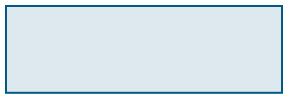
\includegraphics[width=150px]{myndir/heild.png}
\end{center}

Við skilgreindum \hyperlink{row:5227}{stofnbrotið} $\frac1b$ til að svara eftirfarandi spurningu: ``Ef tiltekinni heild er skipt í $b$ jafna hluta, hver er þá stærð hvers hluta miðað við heildina?'' Með öðrum orðum hefur sérhver hluti á myndinni að neðan stærðina $\frac1b$ miðað við heildina:

\begin{center}
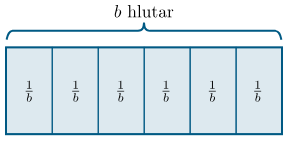
\includegraphics[width=150px]{myndir/b_hlutar.png}
\end{center} 

Hér höfum við áhuga á að svara aðeins almennari spurningu: ``Ef heildinni er skipt í $b$ jafna hluta, hver er þá stærð $a$ slíkra hluta miðað við heildina?'' Til að svara spurningunni innleiðum við táknið $\frac{a}b$, sem við lesum „$a$ á móti $b$“ eða „$a$ $b$-tu“. Við látum sem sagt $\frac{a}b$ tákna stærð dökka svæðisins á myndinni að neðan miðað við heildina:

\begin{center}
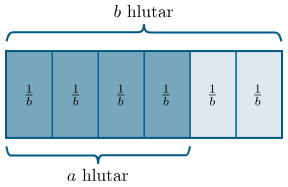
\includegraphics[width=150px]{myndir/a_hlutar.png}
\end{center} &  \\
\hline
273 & \hypertarget{row:273}{andhverfa (vörpunar), andhverf vörpun} & \textit{Andhverfa} \hyperlink{row:3282}{vörpunnar} $f: X \to Y$, ef hún er til, er vörpun $g: Y \to X$ þannig að \hyperlink{row:4518}{samskeyting} varpananna $f$ og $g$ annars vegar og $g$ og $f$ hins vegar sé viðeigandi \hyperlink{row:4498}{samsemdarvörpun}, þ.e. \[ g \circ f = \mathrm{id}_X \quad \text{og} \quad f \circ g = \mathrm{id}_Y. \] Andhverfa $f$ er yfirleitt táknuð með $f^{-1}$ & Ef slík vörpun $g$ er til \hyperlink{row:3932}{ákvarðast hún ótvírætt} af þessum \hyperlink{row:4797}{skilyrðum}. Vörpun $f: X \to Y$ er andhverfanleg ef og aðeins ef hún er \hyperlink{row:1586}{gagntæk}.

Skilyrðin tvö í skilgreiningunni segja með öðrum orðum að fyrir sérhver $x \in X$ og $y \in Y$ gildi að \[ f^{-1}(f(x)) = x \quad \text{og} \quad f(f^{-1}(y)) = y. \] Þetta sýnir að andhverfan $f^{-1}$ hefur einmitt öfuga verkun við $f$, því $f$ varpar \hyperlink{row:5128}{stakinu} $x \in X$ í stakið $f(x) \in Y$ og $f^{-1}$ varpar stakinu $f(x)$ aftur í upphaflega stakið $x$ skv. fyrri jöfnunni. Sömuleiðis hefur $f$ öfuga verkun við $f^{-1}$, því $f^{-1}$ varpar stakinu $y \in Y$ í stakið $f^{-1}(y) \in X$ og $f$ varpar stakinu $f^{-1}(y)$ aftur í upphaflega stakið $y$ skv. seinni \hyperlink{row:2478}{jöfnunni}. Áhrifin af því að beita $f$ og $f^{-1}$ hvorri á eftir annarri eru því engin, sem endurspeglast í \hyperlink{row:6050}{Venn-myndinni} að neðan:

\begin{center}
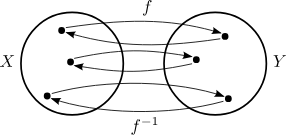
\includegraphics[width=150px]{myndir/andhverfa_vorpunar.png}
\end{center} &  \\
\hline
274 & \hypertarget{row:274}{andhverfanlegur} & \hyperlink{row:3282}{Vörpun} kallast \textit{andhverfanleg} ef hún á sér \hyperlink{row:273}{andhverfu} &  &  \\
\hline
290 & \hypertarget{row:290}{andsælis, rangsælis} &  &  &  \\
\hline
316 & \hypertarget{row:316}{annars stigs margliða, ferningsmargliða} & \hyperlink{row:1948}{Margliða} með stig 2 & Til þess að reikna \hyperlink{row:4254}{rætur} annars stigs margliðu á forminu $ax^2 + bx + c$ má nota \hyperlink{row:2811}{lausnarformúluna}

\[ \frac{-b \pm \sqrt{b^2-4ac}}{2a}. \] 

Þessi formúla er oft kölluð $D$-reglan vegna þess að iðulega er ritað $D=b^2-4ac$ en fjöldi \hyperlink{row:4093}{rauntölulausna} á \hyperlink{row:2478}{jöfnunni} $ax^2 + bx + c=0$ ákvarðast algjörlega af gildinu $D$ sem kallast \textit{aðgreinir} eða \textit{greinir} & Minnast á gælunöfn? \\
\hline
334 & \hypertarget{row:334}{armur} & Sjá \hyperlink{row:2198}{horn} &  &  \\
\hline
351 & \hypertarget{row:351}{átæk vörpun} & \hyperlink{row:3282}{Vörpun} sem hefur allt \hyperlink{row:74}{bakmengið} sem \hyperlink{row:3417}{myndmengi}, þ.e. vörpun $f:X \to Y$ sem uppfyllir $f(X)=Y$ & Fyrir sérhverja vörpun $f: X \to Y$ gildir að $f(X)$ er \hyperlink{row:2098}{hlutmengi} í $Y$, svo til að sýna að $f$ sé átæk nægir að sýna að $Y$ sé líka hlutmengi í $f(X)$. Það er gert með því að sýna að sérhvert \hyperlink{row:5128}{stak} $y \in Y$ sé gildi vörpunarinnar $f$, þ.e. að fyrir sérhvert $y \in Y$ sé til $x \in X$ þannig að $f(x) = y$.

\hyperlink{row:6050}{Venn-myndirnar} að neðan sýna tvær varpanir $f: X \to Y$ og $g: Z \to W$. Vörpunin $f$ er átæk því sérhvert stak í $Y$ er gildi vörpunarinnar $f$. Hins vegar er $g$ ekki átæk því til dæmis er stakið lengst til hægri í $W$ ekki gildi vörpunarinnar $g$:

\begin{center}
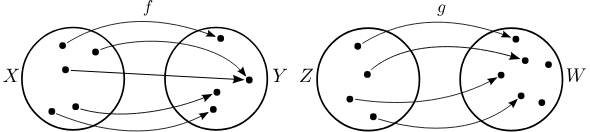
\includegraphics[width=150px]{myndir/ataek_vorpun.png}
\end{center} & Laga stærð á mynd, kannski skipta upp í tvær myndir \\
\hline
363 & \hypertarget{row:363}{áttaður} &  &  &  \\
\hline
419 & \hypertarget{row:419}{baugur} &  &  &  \\
\hline
425 & \hypertarget{row:425}{bein sönnun} & ... &  &  \\
\hline
436 & \hypertarget{row:436}{beint horn} & \hyperlink{row:2198}{Horn} kallast \textit{beint horn} ef \hyperlink{row:334}{armar} þess eru \hyperlink{row:3400}{gagnstæðir}. Slíkt horn \hyperlink{row:2223}{mælist} 180 \hyperlink{row:1667}{gráður} eða $\pi$ \hyperlink{row:478}{radíana} &  & Finna mynd \\
\hline
457 & \hypertarget{row:457}{bil} & \hyperlink{row:2098}{Hlutmengi} $I$ í \hyperlink{row:3270}{mengi} \hyperlink{row:4093}{rauntalna} kallast \textit{bil} ef fyrir sérhver $x, y \in I$ og $z \in \mathbb{R}$ þannig að $x < z < y$ gildi að $z \in I$. Ef mengi rauntalna $a$ þannig að $a \leq x$ fyrir öll $x \in I$ á sér efra mark $L$ kallast $L$ \textit{vinstri endapunktur} bilsins. Sömuleiðis ef mengi rauntalna $b$ þannig að $x \leq b$ fyrir öll $x \in I$ á sér neðra mark $U$ þá kallast $U$ \textit{hægri endapunktur} bilsins & Bil geta verið af ýmsum toga eftir því hvort þau séu með endapunkta (sjá \hyperlink{row:1840}{hálflína}) og hvort þau innihaldi síðan þá endapunkta (sjá \hyperlink{row:3793}{opið bil}, \hyperlink{row:3010}{lokað bil} og \hyperlink{row:1844}{hálfopið bil}). Eftirfarandi tvær myndir sýna allar gerðir bila:

\begin{center}
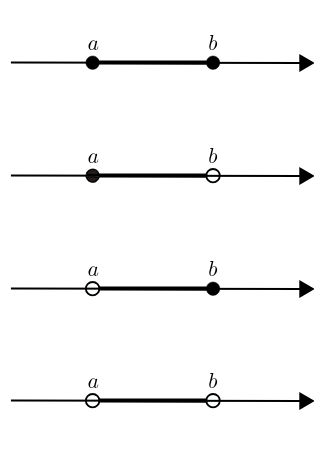
\includegraphics[width=150px]{myndir/takmorkud_bil.png}
\end{center}
\begin{center}
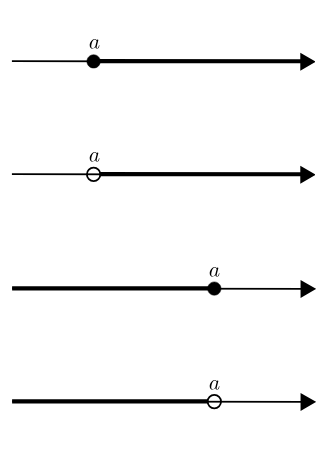
\includegraphics[width=150px]{myndir/otakmorkud_bil.png}
\end{center} & Skoða orðalag, ruglandi að skrifa ``mengi rauntalna $a$'' þegar það sem er meint er ``mengi rauntalna $A$ þannig að $a \leq x$ fyrir öll $a \in A$ \\
\hline
478 & \hypertarget{row:478}{radíani, bogaeining, bogamálseining} & \hyperlink{row:3072}{Mælieining} á \hyperlink{row:5102}{stærð} \hyperlink{row:2198}{horna}. Einn \textit{radíani} er skilgreindur sem stærð hornsins með \hyperlink{row:3661}{oddpunkt} í miðju \hyperlink{row:2295}{hrings} sem fæst þegar að \hyperlink{row:479}{bogalengd} hringsins er jöfn geisla hans & Eftirfarandi mynd sýnir ýmis horn \hyperlink{row:887}{einingarhrings} auk stærð þeirra í bæði gráðum og \hyperlink{row:478}{radíönum}:

\begin{center}
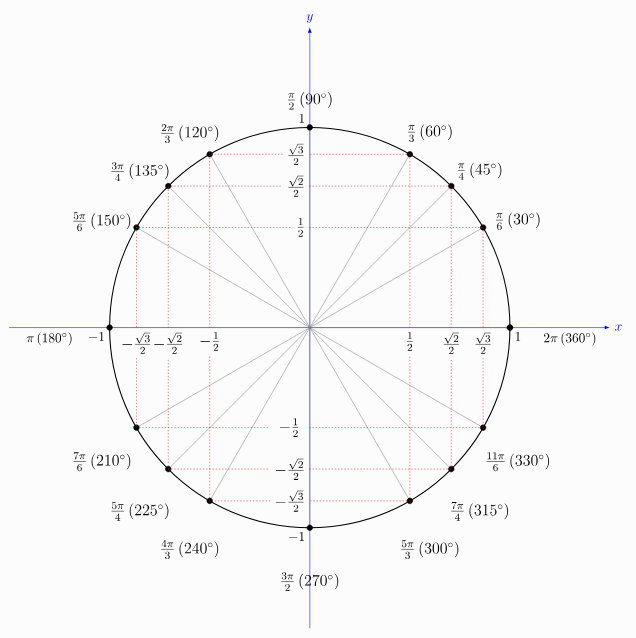
\includegraphics[width=150px]{myndir/hornamal.png}
\end{center} &  \\
\hline
479 & \hypertarget{row:479}{bogalengd} & \hyperlink{row:2860}{Lengd} \hyperlink{row:2276}{hringboga} &  &  \\
\hline
483 & \hypertarget{row:483}{bogamál} &  &  &  \\
\hline
488 & \hypertarget{row:488}{boginn, sveigður} &  &  &  \\
\hline
520 & \hypertarget{row:520}{breiðger rúmfræði} & ... &  &  \\
\hline
538 & \hypertarget{row:538}{breyta, breytistærð, breytileg stærð} & ... &  &  \\
\hline
578 & \hypertarget{row:578}{brún} & \hyperlink{row:2958}{Línustrik} þar sem tvær \hyperlink{row:1325}{hliðar} \hyperlink{row:6454}{þrívíðs} \hyperlink{row:3133}{margflötungs} \hyperlink{row:4771}{skerast} &  & Ræða almenna margflötunga í skýringu? \\
\hline
685 & \hypertarget{row:685}{deiling án afgangs} & \hyperlink{row:686}{Deiling} \hyperlink{row:3475}{náttúrulegrar tölu} með annarri náttúrulegri tölu þar sem afgangurinn er 0 &  &  \\
\hline
686 & \hypertarget{row:686}{deiling með afgangi} & Ef $n$ og $d$ eru \hyperlink{row:1896}{heilar tölur} þannig að $d \neq 0$ þá er til heil tala $q$ og \hyperlink{row:3475}{náttúruleg tala} $r$ sem uppfylla \[n = q \cdot d + r \quad \text{og} \quad 0 \leq r < |d|.\] Að rita $n$ á þessu formi nefnist að \textit{deila} \hyperlink{row:5397}{tölunni} $d$ upp í $n$ og kallast þá talan $q$ \textit{kvóti} deilingarinnar og talan $r$ \textit{afgangur} hennar &  & Óþarfa óþjál skilgreining kannski \\
\hline
722 & \hypertarget{row:722}{dreifinn} & \hyperlink{row:46}{Reikniaðgerð} $\odot$ er sögð vera \textit{dreifin} yfir $\oplus$ ef $\odot$ og $\oplus$ fullnægja \hyperlink{row:723}{dreifireglunni} &  &  \\
\hline
723 & \hypertarget{row:723}{dreifiregla} & Ef $\odot$ og $\oplus$ eru \hyperlink{row:5702}{tvístæðar reikniaðgerðir} á \hyperlink{row:}{mengi} $X$ er sagt að $\odot$ og $\oplus$ fullnægi \textit{dreifireglunni} ef fyrir sérhver \hyperlink{row:5128}{stök} $x, y, z \in X$ gildir að \[ x \odot (y \oplus z) = (x \odot y) \oplus (x \odot z) \] og \[ (y \oplus z) \odot x = (y \odot x) \oplus (z \odot x) \] & Sagt er að $\odot$ og $\oplus$ fullnægi \textit{dreifireglunni frá vinstri} ef fyrir sérhver stök $x, y, z \in X$ gildir að \[ x \odot (y \oplus z) = (x \odot y) \oplus (x \odot z). \] Á sama hátt er sagt að $\odot$ og $\oplus$ fullnægi \textit{dreifireglunni frá hægri} ef fyrir sérhver stök $x, y, z \in X$ gildir að \[ (y \oplus z) \odot x = (y \odot x) \oplus (z \odot x). \] Því er sagt að $\odot$ og $\oplus$ fullnægi dreifireglunni ef $\odot$ og $\oplus$ fullnægi dreifireglunni bæði frá vinstri og hægri. Ef $\odot$ er \hyperlink{row:6228}{víxlin} þá er hún sjálfkrafa dreifin ef hún er dreifin annaðhvort frá hægri eða vinstri &  \\
\hline
737 & \hypertarget{row:737}{eðun} & Fyrir sérhverjar \hyperlink{row:1515}{yrðingar} $p$ og $q$ er $p \vee q$ (lesið: „$p$ eða $q$“) sú yrðing sem segir að að minnsta kosti önnur yrðinganna $p$ og $q$ sé \hyperlink{row:4565}{sönn}. Yrðingin $p \vee q$ er þess vegna \hyperlink{row:3890}{ósönn} þegar yrðingarnar $p$ og $q$ eru báðar ósannar, en annars er hún sönn & Þessari staðreynd má lýsa með töflunni að neðan, sem sýnir sanngildi $p \vee q$ eftir ólíkum sanngildum $p$ annars vegar og $q$ hins vegar & Búa til mynd \\
\hline
759 & \hypertarget{row:759}{eftirfari} &  &  &  \\
\hline
803 & \hypertarget{row:803}{eiginleiki} &  &  &  \\
\hline
832 & \hypertarget{row:832}{einfaldur marghyrningur} &  &  &  \\
\hline
866 & \hypertarget{row:866}{einhalla fall} & \hyperlink{row:1078}{Fall} $f: X \to Y$ þar sem $X$ og $Y$ eru \hyperlink{row:2098}{hlutmengi} í \hyperlink{row:3270}{mengi} \hyperlink{row:4093}{rauntalna} er sagt vera \textit{einhalla} ef það er \hyperlink{row:0}{vaxandi} eða \hyperlink{row:0}{minnkandi} &  & Koma með dæmi um einhalla fall? \\
\hline
884 & \hypertarget{row:884}{einingarferningur} & ... &  &  \\
\hline
887 & \hypertarget{row:887}{einingarhringur} &  &  &  \\
\hline
897 & \hypertarget{row:897}{einliða} & \hyperlink{row:1948}{Margliða} sem hefur aðeins einn lið &  & Koma með dæmi? \\
\hline
922 & \hypertarget{row:922}{einshyrndur} & Tveir \hyperlink{row:6438}{þríhyrningar} kallast \textit{einshyrndir} ef hægt er að para \hyperlink{row:2198}{horn} annars þríhyrningsins við horn hins þríhyrningsins þannig að hornin í sama pari eru \hyperlink{row:2223}{jafn stór} & Á eftirfarandi mynd eru $ABC$ og $FEG$ einshyrndir, táknað $ABC \sim EFG$, vegna þess að:

\begin{enumerate}
    \item $\angle A$ og $\angle E$ eru jafn stór (grænu hornin á myndinni),
    \item $\angle B$ og $\angle F$ eru jafn stór (gulu hornin á myndinni) og
    \item $\angle C$ og $\angle G$ eru jafn stór (rauðu hornin á myndinni).
\end{enumerate}

\begin{center}
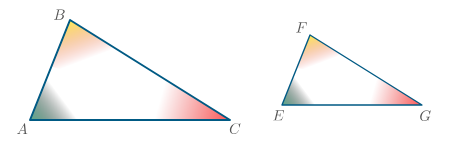
\includegraphics[width=150px]{myndir/einshyrndir_thrihyrningar.png}
\end{center} &  \\
\hline
927 & \hypertarget{row:927}{einskorðun} & Fyrir \hyperlink{row:3282}{vörpun} $f: X \to Y$ kallast vörpunin \[ f|_A : A \to Y; \quad f|_A(x) = f(x) \] þar sem $A$ er \hyperlink{row:2098}{hlutmengi} í $X$ \textit{einskorðun} vörpunarinnar $f$ við mengið $A$ &  &  \\
\hline
932 & \hypertarget{row:932}{einslaga, einslagaður} & Tvær \hyperlink{row:6532}{rúmmyndir} $A$ og $B$ í \hyperlink{row:1034}{evklíðsku rúmi} $\mathbb{E}$ kallast \textit{einslaga} ef til er \hyperlink{row:5779}{færsla} $\phi$ á $\mathbb{E}$ þannig að $\phi(A)$ og $B$ séu \hyperlink{row:0}{eins} rúmmyndir & Á eftirfarandi mynd eru $A$, $B$ og $C$ einslaga:

\begin{center}
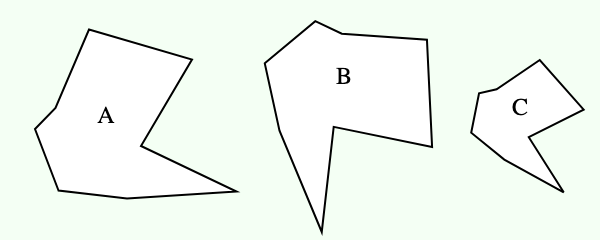
\includegraphics[width=150px]{myndir/einslaga.png}
\end{center} & Laga bakgrunnslit \\
\hline
943 & \hypertarget{row:943}{einslögunarfærsla} & \hyperlink{row:5779}{Færsla} $\phi$ á tiltekinni \hyperlink{row:4884}{sléttu} kallast \textit{einslögunarfærsla} ef \hyperlink{row:2072}{hlutfallið} milli \hyperlink{row:2860}{lengda} \hyperlink{row:2958}{strikanna} $\phi(AB)$ og $AB$ er það sama fyrir öll strik $AB$, sem kallast þá \textit{kvarði} einslögunarfærslunnar &  & Finna mynd \\
\hline
951 & \hypertarget{row:951}{einstæð aðgerð} & \hyperlink{row:46}{Aðgerð} á \hyperlink{row:3270}{mengi} $X$ af gerðinni $X \to X$ kallast \textit{einstæð aðgerð} &  & Koma með dæmi? \\
\hline
963 & \hypertarget{row:963}{einstökungur, einsstaksmengi} & \hyperlink{row:3270}{Mengi} með nákvæmlega eitt \hyperlink{row:5128}{stak} &  & Þarf mynd? \\
\hline
965 & \hypertarget{row:965}{eintæk vörpun} & \hyperlink{row:3282}{Vörpun} sem varpar ólíkum \hyperlink{row:5128}{stökum} úr \hyperlink{row:1343}{formenginu} í ólík stök úr \hyperlink{row:74}{bakmenginu} & Látum $f : X \to Y$ vera vörpun. Í táknmáli segir þessi skilgreining þá að $f$ sé eintæk ef fyrir sérhver $x_1, x_2 \in X$ með $x_1 \neq x_2$ gildir að $f(x_1) \neq f(x_2)$.

Að $f$ varpi ólíkum stökum úr $X$ í ólík stök úr $Y$ má einnig orða svo að ef $f$ varpar tveimur stökum $x_1$ og $x_2$ úr $X$ í sama stakið úr $Y$, þá verði $x_1$ og $x_2$ að vera sama stakið. Með öðrum orðum er $f$ eintæk ef og aðeins ef fyrir sérhver $x_1, x_2 \in X$ með $f(x_1) = f(x_2)$ gildir að $x_1 = x_2$. Þegar sýna á að tiltekin vörpun sé eintæk er oft einfaldara að nota þetta skilyrði en það fyrra.

\hyperlink{row:6050}{Venn-myndirnar} að neðan sýna tvær varpanir $f: X \to Y$ og $g: Z \to W$. Vörpunin $f$ er eintæk því hún varpar ólíkum stökum úr $X$ í ólík stök úr $Y$. Hins vegar er $g$ ekki eintæk því hún varpar tveimur efstu stökunum úr $Z$ í sama stakið í $W$:

\begin{center}
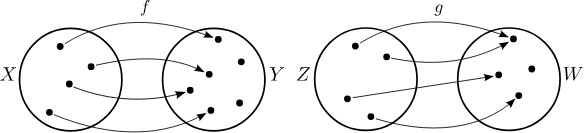
\includegraphics[width=150px]{myndir/eintaek_vorpun.png}
\end{center} & Laga stærð á mynd eða skipta upp í tvær \\
\hline
980 & \hypertarget{row:980}{ekki jákvæður, frekar neikvæður, óviðlægur} &  &  &  \\
\hline
981 & \hypertarget{row:981}{ekki neikvæður, frekar jákvæður, ófrádrægur} &  &  &  \\
\hline
1009 & \hypertarget{row:1009}{endanlegur} & \hyperlink{row:3270}{Mengi} kallast \textit{endanlegt} ef \hyperlink{row:1211}{fjöldatala} þess er \hyperlink{row:3475}{náttúruleg tala} &  &  \\
\hline
1030 & \hypertarget{row:1030}{evklíðsk rúmfræði} & \hyperlink{row:4271}{Rúmfræði} sem byggir á \hyperlink{row:1452}{frumsendum} forngríska \hyperlink{row:5117}{stærðfræðingsins} Evklíðs & Undirstöður rúmfræðinnar má rekja aftur til Evklíðs en í \textit{Frumatriðunum}, sem spanna 13 bækur, tók hann saman alla rúmfræði og \hyperlink{row:5408}{talnafræði} sem þekkt var á þeim tíma. Í fyrstu bókinni setti Evklíð fram fimm frumsendur fyrir rúmfræði í \hyperlink{row:4884}{sléttu} og notaði þær til að leiða út \hyperlink{row:4621}{setningar} um sléttuna. Frumsendur Evklíðs voru fimm talsins:

\begin{enumerate}
    \item Hægt er að teikna beint \hyperlink{row:2958}{strik} milli sérhverra tveggja \hyperlink{row:4001}{punkta}.
    
    \item Hægt er að framlengja sérhvert beint strik í óendanlega langa beina \hyperlink{row:2911}{línu}.

    \item Fyrir strik í sléttu er hægt að draga um það \hyperlink{row:2295}{hring} þannig að strikið sé geisli hringsins, og miðja hans er í öðrum endapunkti striksins.

    \item Öll \hyperlink{row:4167}{rétt horn} eru eins.

    \item Fyrir gefna línu og gefinn punkt, sem ekki er á línunni, er til ein og aðeins ein lína sem fer í gegnum punktinn og \hyperlink{row:4771}{sker} ekki línuna.
\end{enumerate}

Síðasta frumsendan varð eftirmönnum Evklíðs sérstaklega hugleikin og er alltaf vísað í hana sem ``fimmtu frumsendu Evklíðs''. Með því að gera ekki ráð fyrir þessari frumsemdu fæst \hyperlink{row:3705}{óevklíðsk rúmfræði}. &  \\
\hline
1031 & \hypertarget{row:1031}{evklíðsk slétta} & \hyperlink{row:5729}{Tvívítt} \hyperlink{row:4266}{rúm} sem uppfyllir frumsendur \hyperlink{row:1030}{Evklíðskar rúmfræði} &  &  \\
\hline
1040 & \hypertarget{row:1040}{eyðingaraðferð} & ... &  &  \\
\hline
1078 & \hypertarget{row:1078}{fall} & \hyperlink{row:3282}{Vörpun} sem hefur \hyperlink{row:4093}{$\mathbb{R}$} eða \hyperlink{row:5682}{$\mathbb{C}$} sem \hyperlink{row:74}{bakmengi} &  & Koma með dæmi um föll? \\
\hline
1090 & \hypertarget{row:1090}{fallgildi} & Fyrir \hyperlink{row:1078}{fall} $f : X \to Y$ og \hyperlink{row:5128}{stak} $x$ úr $X$ kallast stakið úr $Y$ sem $f$ úthlutar $x$ \textit{gildi fallsins} $f$ í $x$ og táknað með $f(x)$ &  & Þarf mynd? \\
\hline
1125 & \hypertarget{row:1125}{ferflötungur, fjórflötungur, þrístrend strýta, þrístrendur píramíti} & ... &  &  \\
\hline
1127 & \hypertarget{row:1127}{ferhyrningur} & \hyperlink{row:3161}{Marghyrningur} með fjórar \hyperlink{row:2048}{hliðar} & Eftirfarandi er mynd af ferhyrningi:

\begin{center}
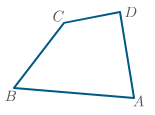
\includegraphics[width=150px]{myndir/ferhyrningur.png}
\end{center} &  \\
\hline
1130 & \hypertarget{row:1130}{ferilhorn} & ... &  &  \\
\hline
1131 & \hypertarget{row:1131}{ferill, boglína, sveiglína} & \hyperlink{row:3417}{Myndmengi} \hyperlink{row:4359}{samfellds falls} á \hyperlink{row:3010}{lokuðu bili} &  & Nota evklíðska skilgreiningu frekar en grannfræðilega? - Finna mynd? \\
\hline
1157 & \hypertarget{row:1157}{ferningsrót, önnur rót} & Ef $a$ er \hyperlink{row:981}{ekki neikvæð} \hyperlink{row:4093}{rauntala} þá er nákvæmlega ein \hyperlink{row:2535}{jákvæð} tala $x$ sem uppfyllir $x^2 = a$ sem er kölluð \textit{kvaðratrótin} af $a$ og táknuð með $\sqrt{a}$ & Kvaðratrót er sértilvik af almenna hugtakinu um \hyperlink{row:4253}{$n$-tu rót} &  \\
\hline
1163 & \hypertarget{row:1163}{ferningur} & \hyperlink{row:4175}{Rétthyrningur} með allar \hyperlink{row:2048}{hliðar} jafn \hyperlink{row:2860}{langar} & Eftirfarandi er mynd af ferningi:

\begin{center}
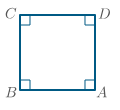
\includegraphics[width=150px]{myndir/ferningur.png}
\end{center} &  \\
\hline
1194 & \hypertarget{row:1194}{firð} & Firð á \hyperlink{row:3270}{mengi} $M$ er \hyperlink{row:1078}{fall} $d:M \times M \to \mathbb{R}_+$, sem uppfyllir 

\begin{itemize}
    \item $d(x,x)=0$ fyrir öll $x \in M$
    \item $d(x,y)>0$ fyrir öll $x \neq y \in M$
    \item $d(x,y)=d(y,x)$ fyrir öll $x,y \in M$
    \item $d(x,y) \leq d(x,z) + d(z,y)$ fyrir öll $x,y,z \in M$
\end{itemize} \hyperlink{row:5102}{Stærðin} $d(x,y)$ er gjarnan kölluð \hyperlink{row:1204}{fjarlægðin} milli $x$ og $y$ &  & Segir ekki skilgreiningin allt sem segja þarf? Er þörf á skýringu? \\
\hline
1200 & \hypertarget{row:1200}{firðrúm} & \hyperlink{row:5627}{Tvennd} $(M,d)$ þar sem $M$ er \hyperlink{row:3270}{mengi} og $d:M \times M \to \mathbb{R}_+$ er \hyperlink{row:1194}{firð} &  & Koma með dæmi um firðrúm? \\
\hline
1204 & \hypertarget{row:1204}{fjarlægð} &  &  &  \\
\hline
1205 & \hypertarget{row:1205}{fjarlægt innra horn} & Þau \hyperlink{row:6295}{innri horn} \hyperlink{row:3161}{marghyrnings} sem ekki eru \hyperlink{row:1677}{grannhorn} tiltekins \hyperlink{row:6295}{ytra horns} & Á eftirfarandi mynd eru $\angle BAC$ og $\angle ACB$ fjarlæg innri horn við ytra hornið $\angle DBC$:

\begin{center}
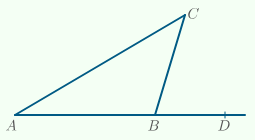
\includegraphics[width=150px]{myndir/ytrahorn.png}
\end{center} & Laga bakgrunnslit \\
\hline
1211 & \hypertarget{row:1211}{fjöldatala} & \hyperlink{row:2489}{Jafngildisflokkur} \hyperlink{row:3270}{mengja} þar sem \hyperlink{row:3332}{milli} sérhverra tveggja \hyperlink{row:3270}{mengja} er til \hyperlink{row:1586}{gagntæk vörpun} &  & Skoða þessa skilgreiningu betur \\
\hline
1229 & \hypertarget{row:1229}{fjölskylda} &  &  &  \\
\hline
1244 & \hypertarget{row:1244}{fjórðungur} & Sjá skýringu við \hyperlink{row:2554}{kartesk hnit} &  &  \\
\hline
1265 & \hypertarget{row:1265}{flatarmál} &  &  &  \\
\hline
1325 & \hypertarget{row:1325}{flötur, hliðarflötur, hlið} & Sjá \hyperlink{row:3133}{margflötungur} &  &  \\
\hline
1328 & \hypertarget{row:1328}{flutningur, hreyfing} & \hyperlink{row:5779}{Færsla} á tiltekinni \hyperlink{row:4884}{sléttu} sem \hyperlink{row:5963}{varðveitir} \hyperlink{row:1204}{fjarlægðir} & Sérhvern flutning má framkvæma með því að nota \hyperlink{row:2056}{hliðrun}, \hyperlink{row:4954}{snúning} og \hyperlink{row:4986}{línuspeglun}. Eins og aðrar færslur, þá varðveita flutningar \hyperlink{row:4509}{samsíða} \hyperlink{row:2911}{línur}. Flutningar varðveita líka \hyperlink{row:2223}{stærðir} \hyperlink{row:2198}{horna} & Finna mynd \\
\hline
1343 & \hypertarget{row:1343}{formengi, frámengi, skilgreiningarmengi, óðal} & Sjá \hyperlink{row:3282}{vörpun} &  &  \\
\hline
1366 & \hypertarget{row:1366}{formynd, frummynd, öfug mynd} & Fyrir \hyperlink{row:3282}{vörpun} $f: X \to Y$ kallast \hyperlink{row:3270}{mengi} þeirra \hyperlink{row:5128}{staka} úr $X$ sem $f$ varpar í stak úr \hyperlink{row:2098}{hlutmengi} $B$ í $Y$ \textit{frummynd} vörpunarinnar $f$ af menginu $B$. Hana má rita á forminu \[ f^{-1}(B) = \{x \in X \mid f(x) \in B\}. \] & Fyrir sérhvert $y \in B$ eru þau stök úr $X$ sem $f$ varpar í $y$ lausnir \hyperlink{row:2478}{jöfnunnar} $f(x) = y$. Frummyndina $f^{-1}(B)$ má því einnig skilgreina sem mengi allra lausna jöfnunnar $f(x) = y$ fyrir sérhvert $y \in B$ og þannig má rita hana á forminu \[ f^{-1}(B) = \{x \in X \mid \text{til er}\; y \in B \;\text{þ.a.}\; f(x) = y\}. \] \hyperlink{row:6050}{Venn-myndin} að neðan sýnir vörpunina $f: X \to Y$, hlutmengið $B$ í $Y$ og frummynd þess $f^{-1}(B)$:

\begin{center}
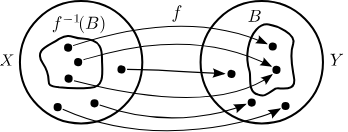
\includegraphics[width=150px]{myndir/frummynd.png}
\end{center}

Frummyndir af \hyperlink{row:4464}{sammengjum}, \hyperlink{row:4928}{sniðmengjum} og \hyperlink{row:1553}{fyllimengjum} fullnægja eftirfarandi \hyperlink{row:4150}{reiknireglum}, sem segja að fyrir sérhver hlutmengi $B_1$ og $B_2$ í $Y$ gildi:

\begin{enumerate}
    \item $f^{-1}(B_1 \cup B_2) = f^{-1}(B_1) \cup f^{-1}(B_2)$.
    \item $f^{-1}(B_1 \cap B_2) = f^{-1}(B_1) \cap f^{-1}(B_2)$.
    \item $f^{-1}(B_1^c) = (f^{-1}(B_1))^c$.
\end{enumerate}

Ef $A$ er hlutmengi í $X$ og $B$ er hlutmengi í $Y$ fást jafnframt eftirfarandi reiknireglur um samspil \hyperlink{row:3417}{mynda} og frummynda:

\begin{enumerate}
    \item $A \subseteq f^{-1}(f(A))$.
    \item $f(f^{-1}(B)) \subseteq B$.
\end{enumerate} &  \\
\hline
1389 & \hypertarget{row:1389}{fótpunktur} &  &  &  \\
\hline
1403 & \hypertarget{row:1403}{frændhorn} & Tvö \hyperlink{row:2198}{horn} sem samanlagt \hyperlink{row:2223}{mælast} 180 \hyperlink{row:1667}{gráður} & Á eftirfarandi mynd eru $\angle BOA$ og $\angle DPC$ frændhorn:

\begin{center}
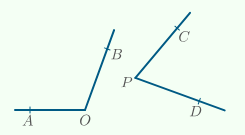
\includegraphics[width=150px]{myndir/fraendhorn.png}
\end{center} & Laga bakgrunnslit \\
\hline
1416 & \hypertarget{row:1416}{framsetning} &  &  &  \\
\hline
1448 & \hypertarget{row:1448}{frumhugtak, grunnhugtak, undirstöðuhugtak} & ... &  &  \\
\hline
1452 & \hypertarget{row:1452}{frumsenda, frumsetning} & \hyperlink{row:1515}{Yrðing} sem lögð er til grundvallar en ekki er ætlast til að sé sönnuð & Í fyrstu gæti virst vafasamt að gefa sér að eitthvað sé \hyperlink{row:6659}{satt} í staðinn fyrir að \hyperlink{row:4554}{sanna} það enda eru \hyperlink{row:4964}{sannanir} aðalverkfæri \hyperlink{row:5117}{stærðfræðinga} til þess að sannfæra sjálfa sig og aðra um að staðhæfingar séu réttar. Því miður er ekki hægt að komast hjá því en það væri eins og að keyra bíl án eldsneytis. Svokölluðu \textit{afleiðslukerfin} sem stærðfræðingar nota er einungis hægt að nota til þess að álykta nýjar staðreyndir út frá staðreyndum sem er nú þegar búið að sanna. Þess vegna þurfa fyrst að vera til staðreyndir sem er ákveðið að séu sannar. Það er ákveðin hætta að frumsendurnar séu innbyrðis \hyperlink{row:3401}{mótsagnakenndar} eða að þær endurspegli ekki innsæi okkar varðandi það sem ætti að vera satt & Ég held að það þurfi að koma með eitthvað dæmi um seinustu setninguna út af hún er ef til vill mjög villandi eins og er \\
\hline
1468 & \hypertarget{row:1468}{frumtala, prímtala} & \hyperlink{row:3475}{Náttúruleg tala} $p > 1$ kallast \textit{frumtala} ef einu náttúrulegu tölurnar sem \hyperlink{row:1599}{ganga upp í} henni eru \hyperlink{row:5397}{talan} $1$ og talan $p$ & Þessi skilgreining jafngildir því að segja að talan $p$ sé frumtala ef fyrir sérhverjar náttúrulegar tölur $a$ og $b$ þannig að $p$ \hyperlink{row:1599}{gengur upp í} $a \cdot b$ þá gengur $p$ líka upp í a.m.k. annarri þeirra.

Ljóst er að fyrsta frumtalan er $2$ og almennt er hægt að ákvarða hvort gefin náttúruleg tala $n$ sé frumtala með því að prófa að \hyperlink{row:686}{deila} öllum frumtölum frá $2$ til $\sqrt{n}$ upp í $n$. Ef alltaf fæst afgangur þá er talan frumtala.

Allar frumtölur minni en 100 eru eftirfarandi: $2, 3, 5, 7, 11, 13, 17, 19, 23, 29, 31, 37, 41, 43, 47, 53, 59, 61, 67, 71, 73, 79, 83, 89, 97$ &  \\
\hline
1475 & \hypertarget{row:1475}{frumþáttur} & Sjá \hyperlink{row:5824}{undirstöðusetningu reikningslistarinnar} &  &  \\
\hline
1515 & \hypertarget{row:1515}{fullyrðing, yrðing} & \hyperlink{row:5072}{Staðhæfing} sem er annaðhvort \hyperlink{row:4565}{sönn} eða \hyperlink{row:3890}{ósönn} & Yrðingar eru yfirleitt táknaðar með litlum bókstöfum eins og $p$, $q$, $r$ og svo framvegis &  \\
\hline
1553 & \hypertarget{row:1553}{fyllimengi} & \hyperlink{row:3280}{Mengjamunur} á forminu $G \setminus A$ þar sem $A \subseteq G$ kallast \textit{fyllimengi} $A$ í $G$. Ef enginn vafi leikur á hvert \hyperlink{row:3270}{mengið} $G$ sé og við höfum ekki áhuga á því sem er utan $G$ (sem kallast þá \textit{grunnmengi}) köllum við þennan mengjamun einfaldlega fyllimengi $A$ og taknum hann með $A^c$ & Ýmis önnur tákn þekkjast fyrir fyllimengi $A$; til dæmis $\overline{A}$, $A’$ og $\mathbf{C}A$. Við höfum sem sagt: \[ A^c = G \setminus A. \] Óformlega má segja að fyllimengið $A^c$ sé sá hluti grunnmengisins sem liggur utan mengisins $A$. Á \hyperlink{row:6050}{Venn-myndum} er venja að tákna grunnmengið með \hyperlink{row:4175}{rétthyrningi}og á myndinni að neðan er fyllimengið $A^c$ litað rautt:

\begin{center}
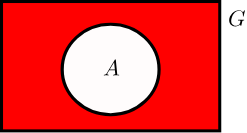
\includegraphics[width=150px]{myndir/fyllimengi.png}
\end{center}

Um fyllimengi \hyperlink{row:4464}{sam-} og \hyperlink{row:4928}{sniðmengja} gilda reglur De Morgans, sem segja að fyrir sérhver tvö mengi $A$ og $B$ gildi: \[ (A \cup B)^c = A^c \cap B^c \quad \text{og} \quad (A \cap B)^c = A^c \cup B^c. \] Jafnframt gilda eftirfarandi reglur fyrir mengin $A$ og $B$:

\begin{enumerate}
    \item $A \cap A^c = \varnothing$.
    \item $A \cup A^c = G$.
    \item $(A^c)^c = A$.
    \item $A \subset B$ ef og aðeins ef $B^c \subset A^c$.
\end{enumerate} &  \\
\hline
1586 & \hypertarget{row:1586}{gagntæk vörpun} & \hyperlink{row:3282}{Vörpun} sem er bæði \hyperlink{row:965}{eintæk} og \hyperlink{row:351}{átæk} & Eftirfarandi mynd sýnir gagntæka vörpun:

\begin{center}
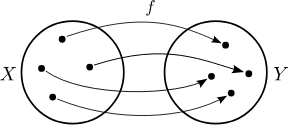
\includegraphics[width=150px]{myndir/gagntaek_vorpun.png}
\end{center} &  \\
\hline
1599 & \hypertarget{row:1599}{ganga upp í} & Sagt er að \hyperlink{row:3475}{náttúruleg tala} $n$ \textit{gengur upp í} náttúrulegri tölu $m$ ef hægt er að \hyperlink{row:685}{deila $m$ með $n$ án afgangs} &  & Koma með dæmi \\
\hline
1616 & \hypertarget{row:1616}{geiri, hringgeiri} & ... &  &  \\
\hline
1619 & \hypertarget{row:1619}{geisli, hringgeisli} & Sjá \hyperlink{row:2295}{hringur} &  &  \\
\hline
1646 & \hypertarget{row:1646}{gleiðhyrndur, sljóhyrndur} & \hyperlink{row:6438}{Þríhyrningur} kallast \textit{gleiðhyrndur} ef hann hefur eitt \hyperlink{row:1647}{gleitt} \hyperlink{row:2198}{horn} & Eftirfarandi mynd sýnir gleiðhyrndan þríhyrning:

\begin{center}
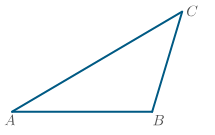
\includegraphics[width=150px]{myndir/gleidhyrndur_thrihyrningur.png}
\end{center} & Laga bakgrunnslit \\
\hline
1647 & \hypertarget{row:1647}{gleiður, sljór} & \hyperlink{row:2198}{Horn} kallast \textit{gleitt} ef það \hyperlink{row:2223}{mælist} stærra en \hyperlink{row:4167}{rétt horn} & Á eftirfarandi mynd er hornið $\angle BOC$ gleitt:

\begin{center}
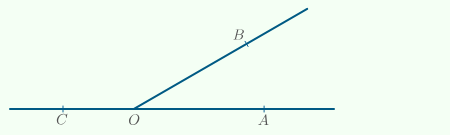
\includegraphics[width=150px]{myndir/hvasst_gleitt.png}
\end{center} &  \\
\hline
1667 & \hypertarget{row:1667}{gráða, horngráða, bogagráða} & \hyperlink{row:3072}{Mælieining} sem oft er notuð til að mæla stærð \hyperlink{row:2276}{hringboga} og \hyperlink{row:2198}{horna} sem er fengin með því að skipta boga hrings í 360 eins boga sem kallast \textit{gráður} og eru táknaðar með $1^\circ$ & Eftirfarandi mynd sýnir ýmis horn \hyperlink{row:887}{einingarhrings} auk stærð þeirra í bæði gráðum og \hyperlink{row:478}{radíönum}:

\begin{center}
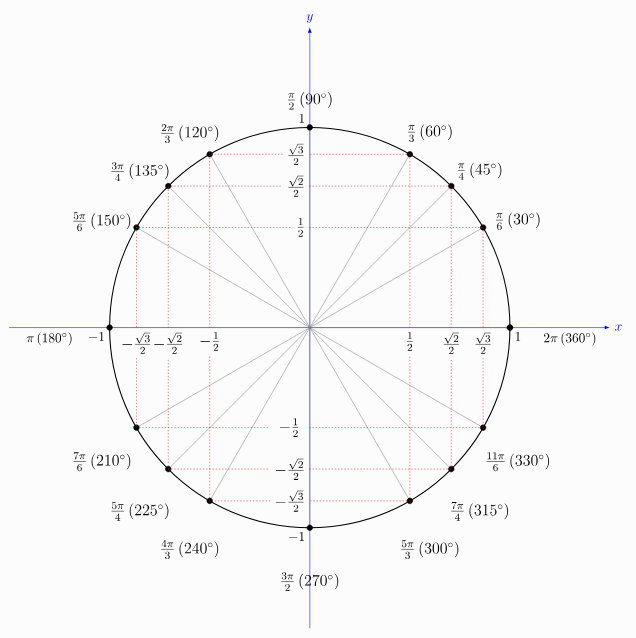
\includegraphics[width=150px]{myndir/hornamal.png}
\end{center} &  \\
\hline
1677 & \hypertarget{row:1677}{grannhorn, aðlæg frændhorn} & Ef tvö \hyperlink{row:2198}{horn} hafa einn sameiginlegan \hyperlink{row:334}{arm} og hinir armarnir eru \hyperlink{row:3400}{gagnstæðar} \hyperlink{row:1840}{hálflínur}, þá er sagt að hornin séu \textit{grannhorn} & Á eftirfarandi mynd eru $\angle COB$ og $\angle BOA$ grannhorn:

\begin{center}
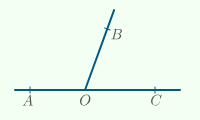
\includegraphics[width=150px]{myndir/grannhorn.png}
\end{center} & Laga bakgrunnslit \\
\hline
1716 & \hypertarget{row:1716}{grunnflötur} & ... &  &  \\
\hline
1723 & \hypertarget{row:1723}{grunnlína} & ... &  &  \\
\hline
1738 & \hypertarget{row:1738}{grunntala, stofntala} & ... &  &  \\
\hline
1757 & \hypertarget{row:1757}{gullinsnið} & ... &  &  \\
\hline
1780 & \hypertarget{row:1780}{hægri dreifiregla} & Sjá \hyperlink{row:723}{dreifiregla} &  &  \\
\hline
1838 & \hypertarget{row:1838}{hálfhringur} &  &  &  \\
\hline
1840 & \hypertarget{row:1840}{hálflína} & \hyperlink{row:457}{Bil} sem hefur nákvæmlega einn endapunkt & Eftirfarandi myndir sýna mismunandi gerðir hálflína:

\begin{center}
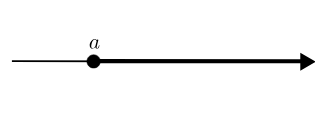
\includegraphics[width=150px]{myndir/lokud_halflina_pos.png}
\end{center}
\begin{center}
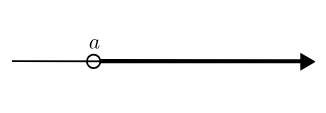
\includegraphics[width=150px]{myndir/opin_halflina_pos.png}
\end{center}
\begin{center}
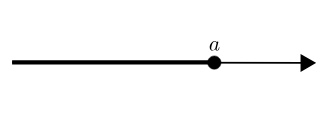
\includegraphics[width=150px]{myndir/lokud_halflina_neg.png}
\end{center}
\begin{center}
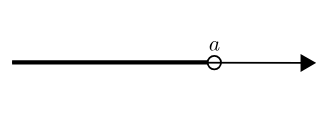
\includegraphics[width=150px]{myndir/opin_halflina_neg.png}
\end{center}

Á fyrstu myndinni má sjá hálflínuna $[a,\infty)$, á annarri myndinni hálflínuna $(a,\infty)$, á þriðju myndinni hálflínuna $(-\infty,a]$ og á seinustu myndinni hálflínuna $(-\infty,a)$ &  \\
\hline
1843 & \hypertarget{row:1843}{hálflokað bil} & Samheiti fyrir \hyperlink{row:1844}{hálfopið bil} &  &  \\
\hline
1844 & \hypertarget{row:1844}{hálfopið bil} & \hyperlink{row:457}{Bil} sem inniheldur nákvæmlega einn endapunkta sinna & Eftirfarandi myndir sína hálfopin bil:

\begin{center}
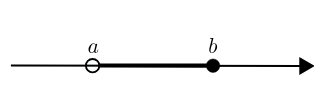
\includegraphics[width=150px]{myndir/halfopid_bil.png}
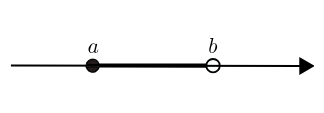
\includegraphics[width=150px]{myndir/halflokad_bil.png}
\end{center}

Á fyrri myndinni inniheldur bilið einungis hægri endapunkt sinn og á síðari myndinni inniheldur bilið einungis vinstri endapunkt sinn & Hálflínur eru samt líka hálfopin bil \\
\hline
1863 & \hypertarget{row:1863}{halli, hallatala} &  &  &  \\
\hline
1896 & \hypertarget{row:1896}{heil tala, heiltala} & \hyperlink{row:3270}{Mengið} $\mathbb{Z}=\mathbb{N} \cup (-\mathbb{N})$ kallast mengi \textit{heillra talna} &  & Þessari skilgreiningu er mjög ábótavant en salta hana í bili \\
\hline
1899 & \hypertarget{row:1899}{heild} &  &  &  \\
\hline
1948 & \hypertarget{row:1948}{heilt rætt fall, margliða} & \hyperlink{row:5097}{Stæða} af gerðinni \[a_{n}x^n + a_{n-1}x^{n-1} + \ldots + a_{1}x + a_{0},\] þar sem $a_{0},\ldots,a_{n}$ eru \hyperlink{row:4093}{rauntölur} og $a_{n} \neq 0$, kallast \textit{margliða}. 

Tölurnar $a_{0}, \ldots, a_{n}$ kallast \textit{stuðlar} margliðunnar og kallast þá $a_{n}$ \textit{forystustuðull} hennar og $a_{0}$ \textit{fastastuðull} hennar. \hyperlink{row:5102}{Stærðirnar} $a_{i}x^i$ kallast \textit{liðir} margliðunnar og kallast þá $a_{n}x^n$ \textit{forystuliður} hennar og $a_{0}$ \textit{fastaliður} hennar.

Talan $n$ kallast \textit{stig} margliðunnar og er það táknað með $\text{deg}(P)$ & Stuðlar margliðu þurfa ekki endilega að vera rauntölur. Almennt þarf \hyperlink{row:3270}{stuðlamengið} bara að vera \hyperlink{row:419}{baugur} & Vantar færslu fyrir fastamargliðu: ``Margliða sem hefur enga liði aðra en fastaliðinn kallast \textit{fastamargliða}'' - Hægt að gera skilgreininguna ennþá kjarnyrtari? \\
\hline
1962 & \hypertarget{row:1962}{helmingalína horns} & \hyperlink{row:2911}{Lína} sem fer í gegnum \hyperlink{row:3661}{oddpunkt} \hyperlink{row:2198}{horns} og skiptir horninu í tvö eins horn kallast \textit{helmingalína hornsins} & Eftirfarandi mynd sýnir helmingalínu hornsins $A$:

\begin{center}
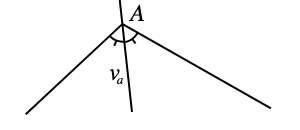
\includegraphics[width=150px]{myndir/helmingalina.png}
\end{center} 

Helmingalínur horna \hyperlink{row:6438}{þríhyrnings} \hyperlink{row:4771}{skerast} allar í einum \hyperlink{row:4001}{punkti} en \hyperlink{row:4845}{skurðpunkturinn} er miðja \hyperlink{row:2418}{innritaðs hrings} þríhyrningsins &  \\
\hline
1974 & \hypertarget{row:1974}{Heronsregla} & Ef \hyperlink{row:6438}{þríhyrningur} hefur \hyperlink{row:0}{hliðarlengdir} $a, b$ og $c$ og $s=\frac{1}{2}(a+b+c)$ er hálft \hyperlink{row:5774}{ummálið}, þá segir \textit{regla Herons} að \hyperlink{row:1265}{flatarmál} þríhyrningsins sé $$ F = \sqrt{s (s - a)(s - b)(s - c)}. $$ & \begin{center}
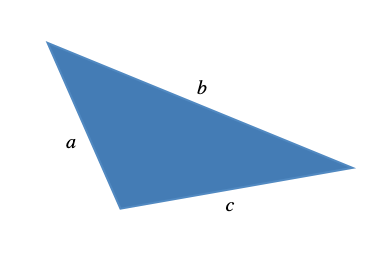
\includegraphics[width=150px]{myndir/heron.png}
\end{center}

Ef þríhyrningurinn hér að ofan hefur hliðarlengdir $a=13$, $b=16$ og $c=21$ þá er $s=25$ og við getum reiknað flatarmálið með \[ F = \sqrt{25\cdot (25-13)\cdot (25-16) \cdot (25-21)}=30\cdot \sqrt{15} \] & Vantar færslu fyrir hliðarlengd \\
\hline
2048 & \hypertarget{row:2048}{hlið, hliðarlína, hliðarstrik} & Sjá \hyperlink{row:3161}{marghyrningur} &  &  \\
\hline
2056 & \hypertarget{row:2056}{hliðrun} & \hyperlink{row:5779}{Færsla} $\tau$ á tiltekinni \hyperlink{row:4884}{sléttu} kallast \textit{hliðrun} ef hún hefur eftirfarandi tvo \hyperlink{row:803}{eiginleika}:

\begin{enumerate}
    \item \hyperlink{row:1204}{fjarlægðin} milli $A$ og $\tau(A)$ er sú sama fyrir alla \hyperlink{row:4001}{punkta} $A$,
    \item ef $A \neq \tau(A)$ gildir fyrir alla punkta $A$ að \hyperlink{row:1840}{hálflínurnar} frá $A$ í gegnum $\tau(A)$ tilgreini sömu \hyperlink{row:5135}{stefnuna}
\end{enumerate} & Hlutlausa færslan telst líka til hliðrana; hún hefur hinsvegar enga tiltekna stefnu. Hliðranir hafa eftirfarandi eiginleika:

\begin{enumerate}
    \item Hliðranir varðveita lengdir allra \hyperlink{row:2958}{strika} og eru því \hyperlink{row:1328}{flutningar}.
    \item Ef $\tau$ er hliðrun, þá eru línurnar $l$ og $\tau(l)$ \hyperlink{row:4509}{samsíða}. Einu flutningarnir sem hafa þennan eiginleika eru hliðranir og \hyperlink{row:0}{punktspeglanir}.
    \item Flutningur sem heldur engum punkti kyrrum er hliðrun.
    \item Samskeyting tveggja hliðrana er hliðrun.
\end{enumerate} & Finna mynd \\
\hline
2072 & \hypertarget{row:2072}{hlutfall} & ... &  & Mismunandi skilgreiningar á ensku og íslensku? \\
\hline
2089 & \hypertarget{row:2089}{hluti, partur} &  &  &  \\
\hline
2098 & \hypertarget{row:2098}{hlutmengi} & \hyperlink{row:3270}{Mengi} $A$ er sagt vera \textit{hlutmengi} í mengi $B$ ef sérhvert \hyperlink{row:5128}{stak} í $A$ er líka stak í $B$. Þetta er táknað með $A \subset B$ & Á \hyperlink{row:6050}{Venn-myndinni} að neðan er $A$ hlutmengi í $B$ því \hyperlink{row:5335}{svæðið} innan minni \hyperlink{row:2295}{hringsins} (sem táknar stökin í $A$) er líka innan stærri hringsins (sem táknar stökin í $B$):

\begin{center}
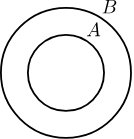
\includegraphics[width=150px]{myndir/hlutmengi.png}
\end{center} & Nota $\subseteq$ í staðinn? \\
\hline
2123 & \hypertarget{row:2123}{hlutur, gripur} &  &  &  \\
\hline
2145 & \hypertarget{row:2145}{hnitakerfi} & \hyperlink{row:4541}{Samsvörun} milli \hyperlink{row:4001}{punkta} tiltekins \hyperlink{row:4266}{rúms} og \hyperlink{row:5397}{talna} sem kallast \textit{hnit} sem gerir manni kleift að staðsetja punkta í rúminu. Slík samsvörun kallast \textit{hnitakerfi} &  & Hægt að skilgreina þetta á formlegri hátt án þess að kafa of djúpt? Endurhugsa aðeins skilgreininguna, hún er ekki mjög skýr - Koma með dæmi um hnitakerfi \\
\hline
2196 & \hypertarget{row:2196}{hópur} &  &  &  \\
\hline
2198 & \hypertarget{row:2198}{horn} & Tvær \hyperlink{row:1840}{hálflínur} með sama \hyperlink{row:5850}{upphafspunkt} eru sagðar mynda \textit{horn}. Upphafspunktur hálflínanna kallast þá \textit{oddpunktur} hornsins og hálflínurnar kallast \textit{armar} þess & Á eftirfarandi mynd sést horn með oddpunkt $O$ og arma $h$ og $k$:

\begin{center}
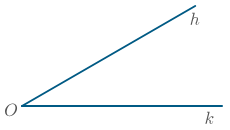
\includegraphics[width=150px]{myndir/horn.png}
\end{center}

Þegar armar horns liggja ekki á sömu \hyperlink{row:2911}{línu}, þá er sagt að hornið sé \textit{eiginlegt}. \hyperlink{row:4001}{Punktur} sem ekki liggur á örmum eiginlegs horns er \textit{innaní} horninu ef hann liggur á \hyperlink{row:2958}{línustriki} með endapunka á örmum þess, en \textit{utanvið} hornið annars. Athugið að sérhver tvö línustrik með sameiginlegan endapunkt sem eru innihaldin í horninu mynda jafnframt sama horn &  \\
\hline
2202 & \hypertarget{row:2202}{hornafall} &  &  &  \\
\hline
2223 & \hypertarget{row:2223}{hornamál} & Til þess að bera saman tvö eiginleg \hyperlink{row:2198}{horn}, þá flytjum við annað hornið þannig að annar armur hornanna sé sameiginlegur og þannig að sérhver \hyperlink{row:4001}{punktur} innaní öðru horninu liggi líka innaní hinu horninu. Þá getur þrennt gerst:

\begin{enumerate}
    \item Hinn armur flutta hornsins fellur saman við hinn arm óhreyfða hornsins. Þá eru hornin \textit{jafn stór}, eða einfaldlega \textit{eins}
    \item Hinn armur flutta hornsins lendir á milli arma óhreyfða hornsins. Þá er flutta hornið minna en óhreyfða hornið, sem er þá jafnframt \textit{stærra} en flutta hornið
    \item Hinn armur flutta hornsins lendir utanvið óhreyfða hornið. Þá er flutta hornið stærra en óhreyfða hornið, sem er þá jafnframt \textit{minna} en flutta hornið
\end{enumerate} & Stærð horns er oft mælt í \hyperlink{row:1667}{gráðum} eða \hyperlink{row:478}{radíönum} &  \\
\hline
2225 & \hypertarget{row:2225}{hornasumma} & \hyperlink{row:2820}{Samanlagt} \hyperlink{row:2223}{gráðumál} \hyperlink{row:2198}{horna} \hyperlink{row:3161}{marghyrnings} Ef \hyperlink{row:2198}{horn} \hyperlink{row:3161}{marghyrnings} eru \hyperlink{row:2223}{mæld} í \hyperlink{row:1667}{gráðum} eða \hyperlink{row:478}{radíönum}, þá er \textit{hornasumma} marghyrnings \hyperlink{row:5320}{summa} stærða allra horna hans & Auðvelt er að finna hornasummu marghyrnings með því að \hyperlink{row:4814}{skipta honum upp í þríhyrninga}. Hægt er að skipta $n$-hyrningi upp í $n-2$ þríhyrninga, svo að hornasumma $n$-hyrnings er $(n-2)\cdot 180$. Sem dæmi er hægt að skipta fimmhyrningnum $A B C D E$ að neðan í þrjá þríhyrninga, svo að hornasumma hans er $(5 - 2) \cdot 180^\circ = 540^\circ$:

\begin{center}
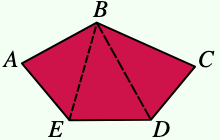
\includegraphics[width=150px]{myndir/hornasumma.png}
\end{center} &  \\
\hline
2235 & \hypertarget{row:2235}{hornpunktur, oddpunktur} & \hyperlink{row:4001}{Punktur} þar sem tvær \hyperlink{row:2048}{hliðar} \hyperlink{row:3161}{marghyrnings} \hyperlink{row:4771}{skerast} (í tveimur \hyperlink{row:6087}{víddum}) eða punktur þar sem þrjár eða fleiri \hyperlink{row:1325}{hliðar} \hyperlink{row:3133}{margflötungs} skerast (í þrem víddum) &  & Ræða almenna margflötunga í skýringu - Þessi skilgreining virkar ekki ef margflötungurinn sker sjálfan sig \\
\hline
2276 & \hypertarget{row:2276}{hringbogi, bogi, örk} & Sá hluti \hyperlink{row:2295}{hrings} sem liggur milli tveggja \hyperlink{row:4001}{punkta} hans kallast \textit{hringbogi} & Á eftirfarandi mynd má sjá hringbogana á milli $A$ og $B$. Sá þessara hringboga sem er innaní \hyperlink{row:2198}{horninu} $\angle AMB$ er dekkri:

\begin{center}
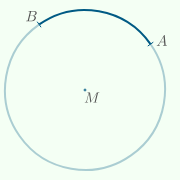
\includegraphics[width=150px]{myndir/hringbogi.png}
\end{center} 

Þegar talað er um bogann $AB$ er jafnan átt við þann minni & Laga bakgrunnslit \\
\hline
2295 & \hypertarget{row:2295}{hringur, hringferill, hringlína} & \hyperlink{row:3270}{Mengi} þeirra \hyperlink{row:4001}{punkta} í tiltekinni \hyperlink{row:4884}{sléttu} sem eru í sömu \hyperlink{row:1204}{fjarlægð} frá punkti sem liggur á sléttunni. Sá punktur kallast þá \textit{miðja} hringsins og fjarlægðin frá honum kallast \textit{geisli} hringsins & Hring með geisla $r$ má einnig skilgreina sem mengi punkta $(x,y)$ sem uppfylla \hyperlink{row:2478}{jöfnuna} \[ x^2+y^2=r^2. \] Eftirfarandi mynd sýnir hring með miðju $M$ og geisla $r$:

\begin{center}
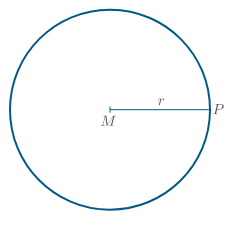
\includegraphics[width=150px]{myndir/hringur.png}
\end{center} &  \\
\hline
2317 & \hypertarget{row:2317}{hvass} & \hyperlink{row:2198}{Horn} kallast \textit{hvasst} ef það \hyperlink{row:2223}{mælist} minna en \hyperlink{row:4167}{rétt horn} & Á eftirfarandi mynd er $\angle AOB$ hvasst horn:

\begin{center}
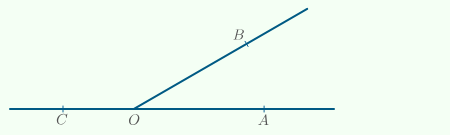
\includegraphics[width=150px]{myndir/hvasst_gleitt.png}
\end{center} & Laga bakgrunnslit \\
\hline
2318 & \hypertarget{row:2318}{hvasshyrndur} & \hyperlink{row:6438}{Þríhyrningur} kallast \textit{hvasshyrndur} ef öll \hyperlink{row:2198}{horn} hans eru \hyperlink{row:2317}{hvöss} & Eftirfarandi mynd sýnir hvasshyrndan þríhyrning:

\begin{center}
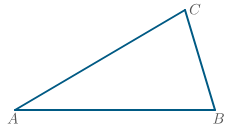
\includegraphics[width=150px]{myndir/hvasshyrndur_thrihyrningur.png}
\end{center} &  \\
\hline
2319 & \hypertarget{row:2319}{hvel, kúluhvel, kúluflötur, kúluyfirborð} & \hyperlink{row:3270}{Mengi} þeirra \hyperlink{row:4001}{punkta} sem eru í sömu \hyperlink{row:1204}{fjarlægð} frá tilteknum punkti. Sá punktur kallast þá
\textit{miðja} kúluhvelsins og fjarlægðin frá honum kallast \textit{geisli} kúluhvelsins & Eftirfarandi er mynd af kúluhveli:

\begin{center}
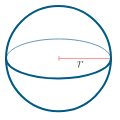
\includegraphics[width=150px]{myndir/kuluhvel.png}
\end{center} & Finna betri mynd \\
\hline
2337 & \hypertarget{row:2337}{hversdagsleg mengjafræði} &  &  &  \\
\hline
2391 & \hypertarget{row:2391}{innhyrndur marghyrningur} & ... &  &  \\
\hline
2418 & \hypertarget{row:2418}{innritaður hringur, innanverður snertihringur} & \hyperlink{row:2295}{Hringur} er \textit{innritaður} í \hyperlink{row:3161}{marghyrning} ef allar \hyperlink{row:2048}{hliðar} marghyrningsins eru \hyperlink{row:4912}{snertlar} við hringinn & Eftirfarandi mynd sýnir þríhyrning með innrituðum hring:

\begin{center}
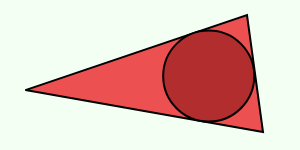
\includegraphics[width=150px]{myndir/innritaður_hringur.png}
\end{center} & Laga bakgrunnslit \\
\hline
2426 & \hypertarget{row:2426}{innsetningaraðferð} & ... &  &  \\
\hline
2453 & \hypertarget{row:2453}{jaðar} &  &  &  \\
\hline
2474 & \hypertarget{row:2474}{jafn, jafnstór} &  &  &  \\
\hline
2478 & \hypertarget{row:2478}{jafna, líking} & \hyperlink{row:1515}{Yrðing} sem lýsir því að tvær \hyperlink{row:5102}{stærðir} séu \hyperlink{row:2474}{jafnar} & Dæmi um jöfnu er staðhæfingin $q(x)$: „$x^2 = 1$“ sem er jafna með óþekktu \hyperlink{row:5102}{stærðina} $x$. Þegar talan $-1$ er sett í stað óþekktu stærðarinnar fæst staðhæfingin $p(-1)$: „$(-1)^2 = 1$“, sem er \hyperlink{row:6659}{sönn} yrðing. Þegar talan $-2$ er sett í stað óþekktu stærðarinnar fæst hins vegar staðhæfingin $p(-2)$: „$(-2)^2 = 1$“, sem er \hyperlink{row:6624}{ósönn} yrðing &  \\
\hline
2480 & \hypertarget{row:2480}{jafnarma} & \hyperlink{row:6438}{Þríhyrningur} kallast \textit{jafnarma} ef hann hefur tvær eins \hyperlink{row:2048}{hliðar} & Eftirfarandi er mynd af jafnarma þríhyrningi:

\begin{center}
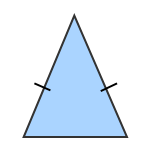
\includegraphics[width=150px]{myndir/jafnarma_thrihyrningur.png}
\end{center} & Finna betri mynd \\
\hline
2489 & \hypertarget{row:2489}{jafngildisflokkur} & \hyperlink{row:2098}{Hlutmengi} $A$ í \hyperlink{row:3270}{mengi} $X$ sem uppfyllir fyrir öll $x,y \in A$ að $x$ og $y$ séu \hyperlink{row:0}{vensluð saman} með tilliti til tiltekinna \hyperlink{row:6592}{jafngildisvensla} og að $x \in A$ sé ekki venslað saman við neitt \hyperlink{row:5128}{stak} í $X \setminus A$ &  & Koma með dæmi (sama og í færslunni um jafngildisvensl? \\
\hline
2496 & \hypertarget{row:2496}{jafnhliða þríhyrningur} & \hyperlink{row:6438}{Þríhyrningur} með allar \hyperlink{row:2048}{hliðar} jafn \hyperlink{row:2860}{langar} & Öll \hyperlink{row:2198}{horn} jafnhliða þríhyrnings eru \hyperlink{row:2223}{jafn stór}, reyndar mælast þau öll $\frac23\pi$ \hyperlink{row:478}{radíana} eða 60 \hyperlink{row:1667}{gráður}. Eftirfarandi er mynd af jafnhliða þríhyrningi:

\begin{center}
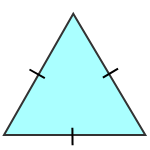
\includegraphics[width=150px]{myndir/jafnhlida_thrihyrningur.png}
\end{center} & Finna betri mynd \\
\hline
2518 & \hypertarget{row:2518}{jafnstæður} & \hyperlink{row:1078}{Fall} $f: X \to Y$ þar sem $X$ og $Y$ eru \hyperlink{row:2098}{hlutmengi} í \hyperlink{row:3270}{mengi} \hyperlink{row:4093}{rauntalna} kallast \textit{jafnstætt} ef fyrir öll $x \in X$ gildi að \[ f(-x) = f(x)\] & \hyperlink{row:2955}{Graf} jafnstæðs falls fellur í sjálft sig við \hyperlink{row:4986}{speglun} um $y$-ásinn. Eftirfarandi mynd sýnir jafnstætt fall:

\begin{center}
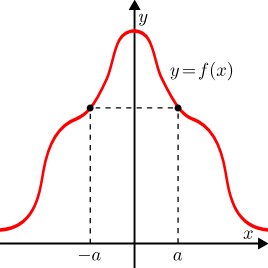
\includegraphics[width=150px]{myndir/jafnstaett_fall.png}
\end{center} &  \\
\hline
2535 & \hypertarget{row:2535}{jákvæður, viðlægur} & \hyperlink{row:4093}{Rauntala} kallast \textit{jákvæð} ef hún er stærri en 0 &  & Vantar færslu fyrir samanburð á rauntölum (samanburður er til en e.t.v. of vítt hugtak) \\
\hline
2546 & \hypertarget{row:2546}{jöfn tala, slétt tala} & \hyperlink{row:1896}{Heil tala} sem $2$ \hyperlink{row:1599}{gengur upp í}, þ.e. heil tala $n$ sem rita má á forminu $n = 2 \cdot k$ þar sem $k$ er heil tala &  &  \\
\hline
2548 & \hypertarget{row:2548}{jöfnuhneppi} & ... &  &  \\
\hline
2554 & \hypertarget{row:2554}{kartesk hnit, Kartesarhnit} & \hyperlink{row:2145}{Hnitakerfi} á \hyperlink{row:1031}{evklíðska sléttu} sem fæst með því að setja upp \hyperlink{row:6469}{þverstæðar} \hyperlink{row:5416}{talnalínur} sem kallast \textit{hnitaásar} og \hyperlink{row:4771}{skerast} í núllpunktum sínum. Þessi \hyperlink{row:4845}{skurðpunktur} kallast þá \textit{upphafspunktur} hnitakerfisins sem er yfirleitt táknaður með $O$ og venja er að kalla aðra talnalínuna $x$-ás og hina $y$-ás & Eftirfarandi er mynd af kartesku hnitakerfi:

\begin{center}
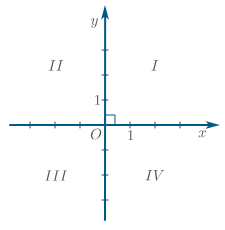
\includegraphics[width=150px]{myndir/kartesk_hnit.png}
\end{center}

Upphafspunkturinn skiptir $x$-ás í tvær \hyperlink{row:1840}{hálflínur}; þá sem hefur \hyperlink{row:4001}{punkta} með \hyperlink{row:981}{frekar jákvæð} hnit og kallast \textit{jákvæði $x$-ás}, og aðra sem hefur punkta með \hyperlink{row:980}{frekar neikvæð} hnit og kallast \textit{neikvæði $x$-ás}. Sama á við um $y$-ás. Jákvæðu ásarnir tilgreina \hyperlink{row:5135}{stefnu} á hnitaásunum. Á mynd er venja að gefa jákvæðu stefnu hnitaásanna til kynna með \hyperlink{row:3810}{ör} og merkja ásana við örina með $x$ eða $y$.

Hnitaásarnir skipta sléttunni í fjóra \textit{fjórðunga}:

\begin{enumerate}
    \item Fyrsti fjórðungur samanstendur af þeim punktum sléttunnar sem eru innaní \hyperlink{row:4167}{rétta horninu} sem hefur jákvæða $x$-ás og jákvæða $y$-ás fyrir \hyperlink{row:334}{arma} sína,

    \item Annar fjórðungur samanstendur af þeim punktum sléttunnar sem eru innaní rétta horninu sem hefur neikvæða $x$-ás og jákvæða $y$-ás fyrir arma sína,

    \item Þriðji fjórðungur samanstendur af þeim punktum sléttunnar sem eru innaní rétta horninu sem hefur neikvæða $x$-ás og neikvæða $y$-ás fyrir arma sína,

    \item Fjórði fjórðungur samanstendur af þeim punktum sléttunnar sem eru innaní rétta horninu sem hefur jákvæða $x$-ás og neikvæða $y$-ás fyrir arma sína,
\end{enumerate}

Þegar sléttan er \hyperlink{row:363}{áttuð} er venja að velja hnitaásana þannig að \hyperlink{row:5145}{stefnuhornið} sem hefur jákvæða $x$-ás sem fyrri arm og jákvæða $y$-ás fyrir seinni arm hafi jákvæða áttun. Þá fæst að þegar jákvæða $x$-ás er \hyperlink{row:4954}{snúið} \hyperlink{row:290}{rangsælis}, þá fer hann fyrst í gegnum fyrsta fjórðung áður en hann fellur í jákvæða $y$-ás. Þegar honum er snúið áfram, þá fer hann næst í gegnum annan fjórðung, þá þriðja og loks fjórða fjórðung.

Með hjálp hnitaásanna má samsama punktum sléttunnar við \hyperlink{row:5627}{tvenndir} af \hyperlink{row:4093}{rauntölum} með eftirfarandi hætti:

\begin{enumerate}
    \item Látum $P$ vera punkt í sléttunni. Látum $A$ vera \hyperlink{row:1389}{fótpunkt} þverilsins á $x$-ás í gegnum $P$. Hnit $A$ á $x$-ásnum er rauntala $a$ sem kallast $x$-hnit $P$. Hún er stundum táknuð $x(P)$. Eins látum við $B$ vera fótpunkt \hyperlink{row:2975}{þverilsins} á $y$-ás í gegnum $P$. Hnit $B$ á $y$-ásnum er rauntala $b$ sem kallast $y$-hnit $P$. Hún er stundum táknuð $y(P)$. Talnatvenndin $(a,b)$ kallast einu nafni \textit{kartesk hnit} punktsins $P$, eða einfaldlega hnit $P$.

    \item Látum $(a,b)$ vera rauntalnatvennd. Látum $A$ er punktinn á $x$-ás sem hefur hnit $a$ og $B$ vera punktinn á $y$-ás sem hefur hnit $b$. Þverillinn á $x$-ás í gegnum punktinn $A$ sker þverilinn á $y$-ás í gegnum punktinn $B$. Látum $P$ vera skurðpunktinn. Stundum er skurðpunkturinn einnig táknaður með $P(a,b)$ til að gefa talnatvenndina til kynna.
\end{enumerate}

\begin{center}
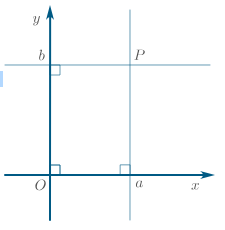
\includegraphics[width=150px]{myndir/kartesk_hnit_b.png}
\end{center} & Er þetta nógu nákvæm skilgreining? \\
\hline
2559 & \hypertarget{row:2559}{kassi, kubbur, rétthyrndur samhliðungur} & \hyperlink{row:4625}{Sexflötungur} þar sem \hyperlink{row:65}{aðlægar hliðar} mynda \hyperlink{row:4167}{rétt horn} & Eftirfarandi er mynd af kassa með hliðarlengdir $l,b$ og $h$:

\begin{center}
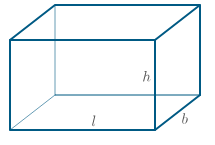
\includegraphics[width=150px]{myndir/kassi.png}
\end{center} &  \\
\hline
2576 & \hypertarget{row:2576}{keila} & \hyperlink{row:6532}{Rúmmynd} sem afmarkast af \hyperlink{row:2579}{fleti} með \hyperlink{row:488}{sveigðum} \hyperlink{row:2453}{jaðri} og \hyperlink{row:2579}{fletinum} sem fæst með því að draga \hyperlink{row:2958}{línustrik} milli \hyperlink{row:4001}{punkta} jaðarins og eins annars punkts &  & Má punkturinn liggja í grunnfletinum? - Óþarfi að vitna í færsluna fyrir keiluflöt út af því það er skilgreint hvernig hann er smíðaður hér? \\
\hline
2579 & \hypertarget{row:2579}{keiluflötur} &  &  &  \\
\hline
2657 & \hypertarget{row:2657}{kósínus} & Fyrir \hyperlink{row:4173}{rétthyrndan þríhyrning} $ABC$ þar sem $C$ er \hyperlink{row:4167}{rétt horn} er \hyperlink{row:2202}{hornafallið} \textit{kósínus} af \hyperlink{row:2198}{horninu} $A$, táknað $\cos(A)$, skilgreint sem \hyperlink{row:2072}{hlutfallið} milli \hyperlink{row:2860}{lengd} \hyperlink{row:65}{aðlægrar} \hyperlink{row:4725}{skammhliðar} og lengd \hyperlink{row:2789}{langhliðar}. Sjá eftirfarandi mynd: 

\begin{center}
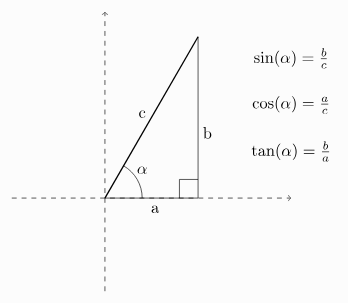
\includegraphics[width=150px]{myndir/hornafoll.png}
\end{center} & Eftirfarandi mynd sýnir hluta \hyperlink{row:2955}{grafs} kósínusarfallsins: 

\begin{center}
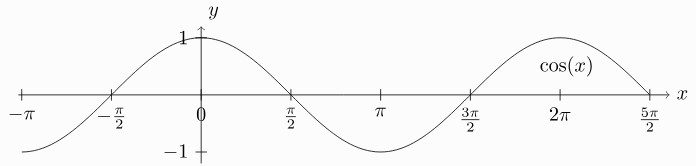
\includegraphics[width=150px]{myndir/cos.png}
\end{center} & Laga nöfn? Laga bakgrunnslit \\
\hline
2658 & \hypertarget{row:2658}{kósínusregla} & Um \hyperlink{row:6438}{þríhyrning} $\Delta A B C$ með \hyperlink{row:0}{hliðarlengdir} $a$, $b$ og $c$ gildir \textit{kósínusreglan} $$ c^2 = a^2 + b^2 - 2 a b\, \cos(C). $$ Þegar \hyperlink{row:2198}{hornið} $C$ er \hyperlink{row:4167}{rétt}, þá er síðasti liðurinn $0$ og \hyperlink{row:2478}{jafnan} gefur \hyperlink{row:4002}{reglu Pýþagórasar} &  & Koma með dæmi? Útskýra hvernig setningunni er beitt? Finna mynd? \\
\hline
2661 & \hypertarget{row:2661}{kótangens} & Fyrir \hyperlink{row:4173}{rétthyrndan þríhyrning} $ABC$ þar sem $C$ er \hyperlink{row:4167}{rétt horn} er \hyperlink{row:2202}{hornafallið} \textit{kótangens} af \hyperlink{row:2198}{horninu} $A$, táknað $\cot(A)$, skilgreint sem \hyperlink{row:2072}{hlutfallið} milli \hyperlink{row:2860}{lengd} \hyperlink{row:65}{aðlægrar} \hyperlink{row:4725}{skammhliðar} og lengd \hyperlink{row:3396}{mótlægrar} skammhliðar & Eftirfarandi mynd sýnir hluta \hyperlink{row:2955}{grafs} kótangensfallsins: 

\begin{center}
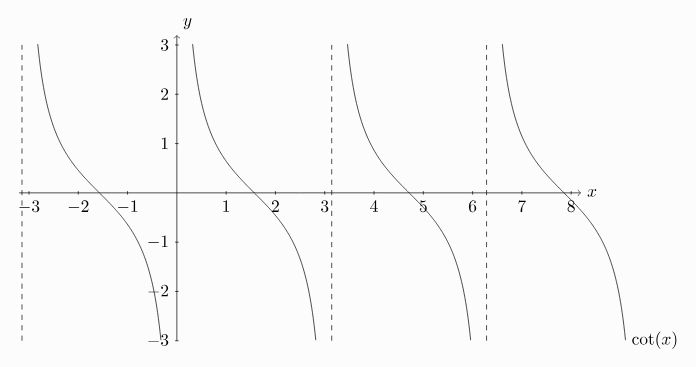
\includegraphics[width=150px]{myndir/cot.png}
\end{center} & Betra að láta táknmál fylgja með? Laga bakgrunnslit - Finna mynd sem skýrir tenginguna við þríhyrning \\
\hline
2680 & \hypertarget{row:2680}{kúla, hnöttur, knöttur} & \hyperlink{row:6532}{Rúmmynd} sem afmarkast af \hyperlink{row:2319}{kúluhveli} &  &  \\
\hline
2682 & \hypertarget{row:2682}{kúlnarúmfræði} & ... &  &  \\
\hline
2717 & \hypertarget{row:2717}{kúptur marghyrningur, úthyrndur marghyrningur} & ... &  &  \\
\hline
2776 & \hypertarget{row:2776}{lagshorn} & Tvö \hyperlink{row:2198}{horn} sem samanlagt \hyperlink{row:2223}{mælast} 90 \hyperlink{row:1667}{gráður} & Á eftirfarandi mynd eru $\angle BOA$ og $\angle COB$ lagshorn:

\begin{center}
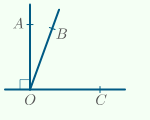
\includegraphics[width=150px]{myndir/lagshorn.png}
\end{center} & Hugtakabankinn segir að hornin þurfa að vera aðlæg en Wikipedia gerir enga slíka kröfu - Laga bakgrunnslit \\
\hline
2781 & \hypertarget{row:2781}{láhnit} & ... &  &  \\
\hline
2789 & \hypertarget{row:2789}{langhlið} & Sú \hyperlink{row:2048}{hlið} \hyperlink{row:}{rétthyrnds þríhyrnings} sem liggur á móti rétta horninu & Á eftirfarandi mynd er $CA$ langhlið þríhyrningsins:

\begin{center}
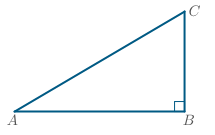
\includegraphics[width=150px]{myndir/retthyrndur_thrihyrningur.png}
\end{center}

Þessi hlið er nefnd langhliðin vegna þess að hún er lengri en báðar hinar hliðarnar. \hyperlink{row:6436}{Þríhyrningsójafnan} segir okkur að $|AB| + |BC| \leq |CA|$ en af því leiðir að ef þríhyrningurinn er ekki \hyperlink{row:5871}{úrkynjaður} þá er $|AB|>0$ og $|BC|>0$ og því gildir $|AB|<|CA|$ og $|BC|<|CA|$ &  \\
\hline
2811 & \hypertarget{row:2811}{lausnarformúla} &  &  &  \\
\hline
2820 & \hypertarget{row:2820}{leggja saman} &  &  &  \\
\hline
2836 & \hypertarget{row:2836}{leiðing} & \hyperlink{row:2836}{Yrðing} af taginu $A \implies B$ kallast \textit{leiðing} en  $A$ kallast þá \textit{skilyrði} og $B$ \textit{ályktun} &  & Koma með dæmi um leiðingar? \\
\hline
2860 & \hypertarget{row:2860}{lengd} &  &  &  \\
\hline
2911 & \hypertarget{row:2911}{lína, bein lína} &  &  &  \\
\hline
2955 & \hypertarget{row:2955}{graf, línurit, fallrit, varprit, ferill (falls)} & Fyrir \hyperlink{row:3282}{vörpun} $f: X \to Y$ kallast \hyperlink{row:3270}{mengi} allra \hyperlink{row:5627}{tvennda} af gerðinni $(x,f(x))$, þar sem $x \in X$ \textit{graf} vörpunarinnar $f$ og er táknað með \[ G_f = \{(x,f(x)) \mid x \in X\} \] & Graf falls $f: X \to Y$, þar sem $X$ og $Y$ eru hlutmengi í mengi \hyperlink{row:4093}{rauntalna}, má teikna í \hyperlink{row:5729}{tvívítt} \hyperlink{row:2145}{hnitakerfi} með því að merkja inn alla \hyperlink{row:4001}{punkta} sem hafa hnit $(x,f(x))$. Þá er venja að merkja grafið með \hyperlink{row:2478}{jöfnunni} $y = f(x)$, því hún lýsir hvernig $y$-hnit punktanna á grafinu fást út frá $x$-hnitum þeirra. Skoðum sem dæmi \hyperlink{row:1078}{fallið} $f: \mathbb{R} \to \mathbb{R}$; $f(x) = x^2$. Graf þess er mengið sem samanstendur af öllum tvenndum af gerðinni $(x,f(x)) = (x,x^2)$ þar sem $x \in \mathbb{R}$, þ.e. \[ G_f = \{(x,x^2) \mid x \in \mathbb{R}\}. \] Eins og lýst er að ofan má teikna grafið í hnitakerfi með því að merkja inn alla punkta sem hafa hnit $(x,x^2)$. Nokkur dæmi um punkta af þessari gerð eru $(-3,9)$, $(-2,4)$, $(-1,1)$, $(0,0)$, $(1,1)$, $(2,4)$ og $(3,9)$. Á myndinni að neðan hefur graf $f$ verið teiknað í hnitakerfi með rauðum lit og eru punktarnir sjö að framan blálitaðir. Grafið er síðan merkt með jöfnunni $y = x^2$:

\begin{center}
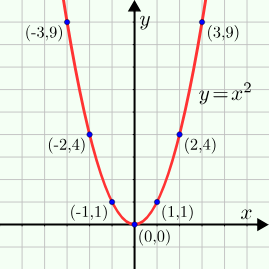
\includegraphics[width=150px]{myndir/graf.png}
\end{center} & Laga bakgrunnslit - Eftirfarandi eru fleiri dæmi um gröf algengra falla: 

Samsemdarvörpunin $f(x) = x$, $x \in \mathbb{R}$:

\begin{center}
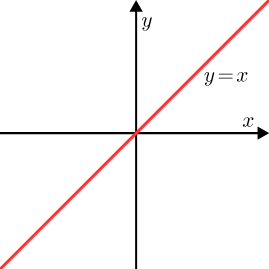
\includegraphics[width=150px]{myndir/graf_samsemdarvorpun.png}
\end{center} - Halda áfram í sama dúr eða láta $x^2$ duga? \\
\hline
2958 & \hypertarget{row:2958}{línustrik, strik} & Sá \hyperlink{row:2089}{hluti} \hyperlink{row:2911}{línu} sem liggur milli tveggja \hyperlink{row:4001}{punkta} sem kallast \textit{endapunktar} línustriksins &  & Finna mynd \\
\hline
2973 & \hypertarget{row:2973}{lóðhnit} & ... &  &  \\
\hline
2975 & \hypertarget{row:2975}{lóðlína, þverlína, þverill} & ... &  &  \\
\hline
3010 & \hypertarget{row:3010}{lokað bil} & \hyperlink{row:457}{Bil} sem inniheldur endapunkta sína & Eftirfarandi er mynd af lokuðu bili:

\begin{center}
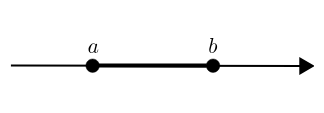
\includegraphics[width=150px]{myndir/lokad_bil.png}
\end{center} &  \\
\hline
3016 & \hypertarget{row:3016}{lokaður ferill, lokaður vegur, lykkja} & \hyperlink{row:1131}{Ferill} þar sem báðir endapunktar ferilsins eru sami punkturinn &  &  \\
\hline
3036 & \hypertarget{row:3036}{lokuð segð, lokuð fullyrðing, lokuð yrðing} & \hyperlink{row:1515}{Yrðing} sem inniheldur engar óþekktar \hyperlink{row:5102}{stærðir} &  &  \\
\hline
3049 & \hypertarget{row:3049}{lotufall, lotubundið fall} & \hyperlink{row:1078}{Fall} $f: \mathbb{R} \to \mathbb{R}$ er sagt vera \textit{lotubundið} ef til er \hyperlink{row:4093}{rauntala} $p > 0$ þannig að fyrir öll $x \in \mathbb{R}$ gildi: \[ f(x + p) = f(x). \] Talan $p$ kallast þá \textit{lota} fallsins & \hyperlink{row:5673}{Tvinngild föll} geta verið lotubundin meðfram \hyperlink{row:5416}{raunásnum} annars vegar eða \hyperlink{row:6473}{þverásnum} hins vegar. Ef fall er lotubundið meðfram báðum ásum kallast það \textit{tvílotubundið} & Þarf skilgreiningarmengið að vera allt $\mathbb{R}$? \\
\hline
3072 & \hypertarget{row:3072}{mælieining} & \textit{Mælieining} er ákveðið \hyperlink{row:3081}{magn} tiltekinnar \hyperlink{row:5102}{stærðar} sem er notað sem viðmið við mælingu slíkra stærða & Mælieiningar eru oft staðlaðar en til að mynda heldur \textit{Bureau international des poids et mesures} (BIPM) utan um SI-einingakerfið sem er mikið notað í vísindum. & Þarf að bæta við að allar mælingar eru þá margfeldi einingarinnar eða setja það í skýringu eða segir það sig kannski sjálft? - Koma með dæmi um mælieiningar \\
\hline
3081 & \hypertarget{row:3081}{magn} &  &  &  \\
\hline
3118 & \hypertarget{row:3118}{margfeldi} &  &  &  \\
\hline
3133 & \hypertarget{row:3133}{margflötungur, flötungur} &  &  & ``<ref idTerm=6532>Rúmmynd</ref> sem samanstendur af <ref idTerm=1009>endanlega</ref> mörgum <ref idTerm=3161>marghyrningum</ref> sem kallast \textit{hliðar} margflötungsins'' Þarf aðeins að endurhugsa skilgreininguna \\
\hline
3141 & \hypertarget{row:3141}{margföldun} &  &  &  \\
\hline
3161 & \hypertarget{row:3161}{marghyrningur, hyrningur} & \hyperlink{row:4891}{Flatarmynd} sem samanstendur af \hyperlink{row:1009}{endanlega} mörgum \hyperlink{row:2958}{línustrikum} (sem kallast \textit{hliðar} marghyrningsins) þannig að sérhvert línustrik deili endapunkti með nákvæmlega einu öðru línustriki & Hugtakið marghyrningur er oft notað til að vísa í \hyperlink{row:832}{einfalda marghyrninga} en almennt mega hliðar marghyrnings skera hvor aðra &  \\
\hline
3270 & \hypertarget{row:3270}{mengi} & \hyperlink{row:4308}{Safn} \hyperlink{row:5114}{hluta} & Þessi skilgreining á mengi skilgreinir svokallaða \hyperlink{row:2337}{hversdagslega mengjafræði} sem ekki er unnt að nota í stærðfræði vegna þess að hún leiðir til mótsagnar (samanber \hyperlink{row:4294}{þversögn Russell}). Sú mengjafræði sem er mest notuð nú til dags er mengjafræðin sem byggir á frumsendum Ernst Zermelo og Abraham Fraenkel og kölluð \hyperlink{row:6314}{Zermelo-Fraenkel-mengjafræði} eða ZF. Oft er einnig gert ráð fyrir \hyperlink{row:5954}{valfrumsendunni} og þá talað um \hyperlink{row:6315}{Zermelo-Fraenkel-mengjafræði með valfrumsendu} eða ZFC &  \\
\hline
3275 & \hypertarget{row:3275}{mengjafræði} &  &  &  \\
\hline
3279 & \hypertarget{row:3279}{mengjamargfeldi, faldmengi, Kartesarmargfeldi, karteskt margfeldi} & \textit{Faldmengi} tveggja \hyperlink{row:3270}{mengja} $X$ og $Y$, táknað $X \times Y$, er mengi \hyperlink{row:5627}{para} $(x,y)$ þannig að $x \in X$ og $y \in Y$ & Almennt ef $I \subseteq \mathbb{N}$ er \hyperlink{row:457}{bil} og $\left(X_i\right)_{i \in I}$ er \hyperlink{row:3684}{runa} af mengjum þá er faldmengi þeirra skilgreint sem mengi runa $(x_i)_{i \in I}$ þannig að $x_i \in X_i$ fyrir öll $i \in I$ &  \\
\hline
3280 & \hypertarget{row:3280}{mengjamunur, mengjamismunur} & \textit{Mengjamunur} tveggja \hyperlink{row:3270}{mengja} $A$ og $B$ er mengi þeirra \hyperlink{row:5128}{staka} sem eru í $A$ en ekki í $B$. Þetta mengi er táknað með $A \setminus B$ (lesið: $A$ án $B$) og það má rita á forminu \[ A \setminus B = \{x \in A \mid x \notin B\}. \] & Óformlega má segja að mengjamunurinn $A \setminus B$ sé sá hluti mengisins $A$ sem er utan mengisins $B$ og á \hyperlink{row:6050}{Venn-myndinni} hér að neðan er hann litaður rauður:

\begin{center}
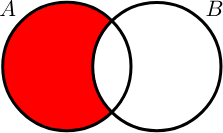
\includegraphics[width=150px]{myndir/mengjamunur.png}
\end{center}

Fyrir öll mengi $A$ og $B$ má rita mengjamuninn $A \setminus B$ sem \hyperlink{row:4928}{sniðmengi} $A$ og \hyperlink{row:1553}{fyllimengis} $B$, þ.e. \[ A \setminus B = A \cap B^c. \] Jafnframt gildir fyrir öll mengi $A$ að $A \setminus \varnothing = A$ og $A \setminus A = \varnothing$ &  \\
\hline
3282 & \hypertarget{row:3282}{vörpun} & \textit{Vörpun} $f: X \to Y$ frá \hyperlink{row:3270}{mengi} $X$ yfir í mengið $Y$ er forskrift eða regla sem úthlutar sérhverju \hyperlink{row:5128}{staki} úr $X$ nákvæmlega einu staki úr $Y$. Mengið $X$ kallast \textit{skilgreiningarmengi} vörpunarinnar og mengið $Y$ kallast \textit{bakmengi} hennar & Í \hyperlink{row:3275}{mengjafræði} er vörpun $f : X \to Y$ skilgreind sem \hyperlink{row:6051}{vensl} sem uppfylla eftirfarandi tvö \hyperlink{row:4797}{skilyrði}:

\begin{enumerate}
    \item Sérhvert stak $x \in X$ er \hyperlink{row:0}{venslað við} eitthvert stak $y \in Y$
    \item Ef $x \in X$ er venslað við $y \in Y$ og $x$ er einnig venslað við $z \in Y$, þá gildir $y = z$ 
\end{enumerate}

Fyrra skilyrðið tryggir að vörpunin sé skilgreind á öllu \hyperlink{row:1343}{formengi} sínu og seinna skilyrðið tryggir það að vörpunin taki ekki mörg \hyperlink{row:5968}{gildi} í einum \hyperlink{row:4001}{punkti} &  \\
\hline
3304 & \hypertarget{row:3304}{miðja, miðdepill, miðpunktur} &  &  &  \\
\hline
3317 & \hypertarget{row:3317}{miðlína} & ... &  &  \\
\hline
3319 & \hypertarget{row:3319}{miðpunktur} & ... &  &  \\
\hline
3325 & \hypertarget{row:3325}{miðstrengur} & Sjá \hyperlink{row:5261}{strengur} &  &  \\
\hline
3328 & \hypertarget{row:3328}{miðþverill, miðþverlína} & ... &  &  \\
\hline
3332 & \hypertarget{row:3332}{milli, á milli} &  &  &  \\
\hline
3347 & \hypertarget{row:3347}{minni, smærri} &  &  &  \\
\hline
3353 & \hypertarget{row:3353}{minnsta samfeldi, minnsta sameiginlega margfeldi} & \hyperlink{row:3347}{Minnsta} \hyperlink{row:3475}{náttúrulega talan} sem tvær \hyperlink{row:1896}{heiltölur} $n$ og $m$ \hyperlink{row:1599}{ganga upp í} kallast \textit{minnsta} \hyperlink{row:4343}{\textit{samfeldi}} $n$ og $m$ og er táknað með $\text{lcm}(n,m)$ & Til þess að finna minnsta samfeldi talna $n$ og $m$ er byrjað á að \hyperlink{row:5824}{frumþátta} þær. Ef $p_{1},\ldots,p_{k}$ eru allir þeir frumþættir sem tilheyra að minnsta kosti annarri tölunni $n$ eða $m$, og $a_{1},\ldots,a_{k}$ og $b_{1},\ldots,b_{k}$ eru margfeldni þeirra í $n$ og $m$, þá er minnsta samfeldi þeirra:

\[ \text{lcm}(n,m) = {p_{1}}^{c_{1}} \cdot {p_{2}}^{c_{2}} \cdot \ldots \cdot {p_{k-1}}^{c_{k-1}} \cdot {p_{k}}^{c_{k}} \] 

þar sem $c_{i}=\max\{a_{i}, b_{i}\}$ &  \\
\hline
3396 & \hypertarget{row:3396}{mótlæg hlið, öndverð hlið, gagnstæð hlið} &  &  &  \\
\hline
3398 & \hypertarget{row:3398}{mótlægt horn} & Sjá \hyperlink{row:5568}{gagnstæð horn} &  &  \\
\hline
3400 & \hypertarget{row:3400}{mótlægur, mótstæður, gagnstæður, öndverður, andstæður, öfugur} &  &  &  \\
\hline
3401 & \hypertarget{row:3401}{mótsagnakenndur, í mótsögn} &  &  &  \\
\hline
3402 & \hypertarget{row:3402}{mótskilyrðing} & ... &  &  \\
\hline
3417 & \hypertarget{row:3417}{myndmengi, mynd} & Fyrir \hyperlink{row:3282}{vörpun} $f: X \to Y$ kallast \hyperlink{row:3270}{mengi} allra \hyperlink{row:5968}{gilda} sem vörpunin tekur \textit{mynd} vörpunarinnar $f$. Hana má rita á forminu \[ f(X) = \{ f(x) \in Y \mid x \in X \}. \] & Myndina $f(X)$ má einnig skilgreina sem mengi allra $y \in Y$ þannig að \hyperlink{row:2478}{jafnan} $y = f(x)$ hafi lausn úr $X$ og þannig má rita hana á forminu \[ f(X) = \{y \in Y \mid \text{til er}\; x \in X \;\text{þ.a.}\; y = f(x)\}. \] \hyperlink{row:6050}{Venn-myndin} að neðan sýnir vörpunina $f: X \to Y$ og mynd hennar $f(X)$:

\begin{center}
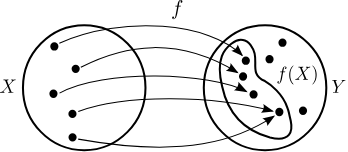
\includegraphics[width=150px]{myndir/myndmengi.png}
\end{center}

Myndin $f(X)$ er alltaf \hyperlink{row:2098}{hlutmengi} í bakmenginu $Y$, en eins og Venn-myndin sýnir þurfa þau ekki að vera \hyperlink{row:2474}{jöfn}, þ.e. til geta verið \hyperlink{row:5128}{stök} í bakmenginu sem eru ekki í myndinni. Með sama móti má tala um mynd vörpunar af hlutmengi í skilgreiningarmenginu. Ef $A \subseteq X$ þá kallast mengi allra gilda sem $f$ tekur á menginu $A$ (táknað með $f(A)$) mynd vörpunarinnar $f$ af menginu $A$. Hana má rita á forminu \[ f(A) = \{f(x) \in Y \mid x \in A\}. \] Venn-myndin að neðan sýnir vörpunina $f: X \to Y$, hlutmengið $A$ í $X$ og mynd þess $f(A)$:

\begin{center}
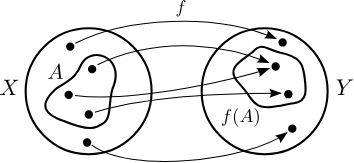
\includegraphics[width=150px]{myndir/myndhlutmengi.png}
\end{center}

Myndir af \hyperlink{row:4464}{sammengjum} og \hyperlink{row:4928}{sniðmengjum} fullnægja eftirfarandi \hyperlink{row:4150}{reiknireglum}, sem segja að fyrir sérhver hlutmengi $A_1$ og $A_2$ í $X$ gildi:

\begin{enumerate}
    \item $f(A_1 \cup A_2) = f(A_1) \cup f(A_2)$
    \item $f(A_1 \cap A_2) \subseteq f(A_1) \cap f(A_2)$
\end{enumerate}

Ef $A$ er hlutmengi í $X$ og $B$ er hlutmengi í $Y$ fást jafnframt eftirfarandi reiknireglur um samspil mynda og \hyperlink{row:1366}{frummynda}:

\begin{enumerate}
    \item $A \subseteq f^{-1}(f(A))$
    \item $f(f^{-1}(B)) \subseteq B$
\end{enumerate} &  \\
\hline
3475 & \hypertarget{row:3475}{náttúrleg tala} & \hyperlink{row:5128}{Stak} í \hyperlink{row:3270}{menginu} $\{0, 1, 2, \dots\}$ (stundum er \hyperlink{row:5397}{talan} \hyperlink{row:3549}{0} ekki tekin með), táknað með $\mathbb{N}$ & Fyrsta tilraun til að skilgreina náttúrulegar tölur formlega var gerð af ítalska \hyperlink{row:5117}{stærðfræðingnum} Giuseppe Peano árið 1889. Hann setti fram eftirfarandi fimm \hyperlink{row:1452}{frumsendur}:

\begin{enumerate}
    \item \textit{Núll} er náttúruleg tala, táknuð með 0
    \item Sérhver náttúruleg tala $n$ á sér \hyperlink{row:759}{eftirfara} sem er náttúruleg tala, táknað með $S(n)$
    \item Núll er ekki eftirfari neinnar náttúrulegrar tölu, það er að segja $0 \neq S(n)$ fyrir neina náttúrulega tölu $n$
    \item Ef eftirfarar tveggja náttúrulegra talna $n$ og $m$ eru jafnir, þá eru $n$ og $m$ jafnar, í táknmáli $S(n)=S(m)\implies n=m$
    \item Ef mengi inniheldur núll og það að náttúruleg tala $n$ sé innihaldin í menginu hafi í för með sér að $S(n)$ sé einnig innihaldið í menginu, þá inniheldur mengið náttúrulegu tölurnar
\end{enumerate}

Seinasta frumsendan er kölluð \textit{þrepunarfrumsendan} en hún gerir okkur kleift að tala um \hyperlink{row:803}{eiginleika} allra náttúrulegra talna (sem eru óendanlega margar) í endanlega mörgum skrefum. Ef $P : \mathbb{N} \to \{\bot,\top\}$ er \hyperlink{row:3800}{opin yrðing} og við skoðum mengið \[ X = \{ n \in \mathbb{N} \mid P(n)\} \] þá segir frumsendan að ef $P(0)$ sé \hyperlink{row:6659}{sönn} og $P(S(n))$ sé sönn að því gefnu að $P(n)$ sé sönn fyrir einhverja náttúrulega tölu $n$, þá er $X = \mathbb{N}$ og þar með gildir $P$ fyrir allar náttúrulegar tölur &  \\
\hline
3497 & \hypertarget{row:3497}{nefnari} & Sjá \hyperlink{row:234}{almennt brot} &  &  \\
\hline
3507 & \hypertarget{row:3507}{neitun} & Fyrir sérhverja \hyperlink{row:1515}{yrðingu} $p$ er $\neg p$ (lesið: „ekki $p$“) sú yrðing sem fæst með því að \textit{neita} yrðingunni $p$. Yrðingin $\neg p$ hefur þess vegna alltaf öfugt \hyperlink{row:4560}{sanngildi} við yrðinguna $p$ & Þessari staðreynd má lýsa með eftirfarandi töflu, sem sýnir \hyperlink{row:4560}{sanngildi} $\neg p$ eftir ólíkum sanngildum $p$: & Búa til mynd \\
\hline
3517 & \hypertarget{row:3517}{niðurstaða, ályktun, lokaályktun} & Sjá \hyperlink{row:2836}{leiðing} &  &  \\
\hline
3563 & \hypertarget{row:3563}{núllmargliða} & \hyperlink{row:0}{Fastamargliðan} 0 kallast \textit{núllmargliðan}. &  &  \\
\hline
3640 & \hypertarget{row:3640}{óbein sönnun} & ... &  &  \\
\hline
3659 & \hypertarget{row:3659}{oddatala, ójöfn tala, hvöss tala} & \hyperlink{row:1896}{Heil tala} sem $2$ \hyperlink{row:1599}{gengur ekki upp í}, þ.e. heil tala $n$ sem rita má á forminu $n = 2 \cdot k + 1$ þar sem $k$ er heil tala &  &  \\
\hline
3661 & \hypertarget{row:3661}{oddpunktur, topppunktur, broddur} & Sjá \hyperlink{row:2198}{horn} &  &  \\
\hline
3663 & \hypertarget{row:3663}{oddstæður} & \hyperlink{row:1078}{Fall} $f: X \to Y$ þar sem $X$ og $Y$ eru \hyperlink{row:2098}{hlutmengi} í \hyperlink{row:3270}{mengi} \hyperlink{row:4093}{rauntalna} kallast \textit{oddstætt} ef fyrir öll $x \in X$ gildi að \[ f(-x) = - f(x). \] & \hyperlink{row:2955}{Graf} oddstæðs falls fellur í sjálft sig þegar því er \hyperlink{row:4986}{speglað} um \hyperlink{row:6253}{$y$-ásinn} og spegilmyndinni síðan speglað um \hyperlink{row:6252}{$x$-ásinn}. Þetta má einnig orða svo að graf oddstæðs falls falli í sjálft sig ef því er snúið um \hyperlink{row:1838}{hálfhring}. Eftirfarandi mynd sýnir oddstætt fall:

\begin{center}
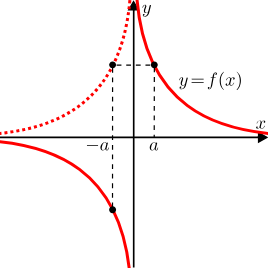
\includegraphics[width=150px]{myndir/oddstaett_fall.png}
\end{center} &  \\
\hline
3684 & \hypertarget{row:3684}{óendanleg runa, runa} &  &  &  \\
\hline
3698 & \hypertarget{row:3698}{óendanlegur} & \hyperlink{row:3270}{Mengi kallast \textit{óendanlegt} ef það er ekki }\hyperlink{row:1009}{endanlegt} &  & Tala um teljanleika \\
\hline
3705 & \hypertarget{row:3705}{óevklíðsk rúmfræði} &  &  &  \\
\hline
3710 & \hypertarget{row:3710}{ofanvarp} & ... &  &  \\
\hline
3744 & \hypertarget{row:3744}{ogun} & Fyrir sérhverjar \hyperlink{row:1515}{yrðingar} $p$ og $q$ er $p \wedge q$ (lesið: „$p$ \textit{og} $q$“) sú yrðing sem segir að $p$ og $q$ séu báðar \hyperlink{row:4565}{sannar}. Yrðingin $p \wedge q$ er þess vegna sönn þegar yrðingarnar $p$ og $q$ eru báðar sannar, en annars er hún \hyperlink{row:3890}{ósönn} & Þessu má lýsa með eftirfarandi töflu, sem sýnir \hyperlink{row:4560}{sanngildi} yrðingarinnar $p \wedge q$ eftir ólíkum sanngildum $p$ annars vegar og $q$ hins vegar: 

\begin{center}
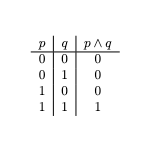
\includegraphics[width=150px]{myndir/ogun.png}
\end{center} & Búa til mynd í betri gæðum \\
\hline
3793 & \hypertarget{row:3793}{opið bil} & \hyperlink{row:457}{Bil} sem inniheldur ekki endapunkta sína & Eftirfarandi er mynd af opnu bili:

\begin{center}
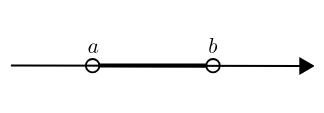
\includegraphics[width=150px]{myndir/opid_bil.png}
\end{center} & Opnar hálflínur eru líka opin bil \\
\hline
3800 & \hypertarget{row:3800}{opin segð, opin fullyrðing, opin yrðing} & \hyperlink{row:1515}{Yrðing} sem inniheldur eina eða fleiri óþekktar \hyperlink{row:5102}{stærðir} & Staðhæfingin $p(x)$: ``$x$ er \hyperlink{row:2546}{slétt tala}'' er opin yrðing með óþekktu stærðina $x$. Þegar talan 1 er sett í stað óþekktu stærðarinnar fæst staðhæfingin $p(1)$: ``1 er slétt tala'', sem er \hyperlink{row:6624}{ósönn} yrðing. Þegar talan 2 er sett í stað óþekktu stærðarinnar fæst hins vegar staðhæfingin $p(2)$: ``$2$ er slétt tala'', sem er \hyperlink{row:6659}{sönn} yrðing. 

Látum $p(x)$ vera opna yrðingu og $X$ vera \hyperlink{row:3270}{mengi}. Þau \hyperlink{row:5128}{stök} úr $X$ sem gera $p(x)$ að sannri yrðingu þegar þau eru sett í stað óþekktu stærðarinnar kallast \textit{lausnir} opnu yrðingarinnar $p(x)$ í menginu $X$. Ennfremur kallast mengi allra lausna $p(x)$ í $X$ \textit{lausnamengi} $p(x)$ í $X$ og það er táknað með \[ P = \{x \in X \mid p(x)\} \] &  \\
\hline
3810 & \hypertarget{row:3810}{ör, píla} &  &  &  \\
\hline
3814 & \hypertarget{row:3814}{óræður} & \hyperlink{row:4093}{Rauntala} kallast \textit{óræð} ef hún er ekki \hyperlink{row:4039}{ræð} &  & Koma með dæmi, til dæmis $\sqrt{2}$ ? \\
\hline
3932 & \hypertarget{row:3932}{ótvírætt ákvarðaður} & \hyperlink{row:5102}{Stærð} $A$ kallast \textit{ótvírætt ákvörðuð} af tilteknum \hyperlink{row:4797}{skilyrðum} ef hún

\begin{enumerate}
    \item uppfyllir þau skilyrði ($A$ er \textit{ákvörðuð} af skilyrðunum),
    \item ef önnur stærð $B$ uppfyllir sömu skilyrði þá gildir $A=B$
\end{enumerate} &  &  \\
\hline
3976 & \hypertarget{row:3976}{pí (\(\pi\))} & ... &  &  \\
\hline
3991 & \hypertarget{row:3991}{prósenta} & ... &  &  \\
\hline
4001 & \hypertarget{row:4001}{punktur, depill} &  &  &  \\
\hline
4002 & \hypertarget{row:4002}{Pýþagórasarregla, setning Pýþagórasar} & \textit{Setning Pýþagórasar} segir að fyrir \hyperlink{row:4173}{rétthyrndan þríhyrning} með \hyperlink{row:0}{hliðarlengdir} $a,b$ og $c$ þar sem $c$ er lengd \hyperlink{row:2789}{langhliðarinnar} gildi \[c^2 = a^2 + b^2\] &  &  \\
\hline
4009 & \hypertarget{row:4009}{raðað mengi, raðmengi, hlutraðað mengi, hlaðmengi} &  &  &  \\
\hline
4039 & \hypertarget{row:4039}{ræð tala} & \hyperlink{row:4093}{Rauntala} sem er hægt að rita sem \hyperlink{row:234}{almennt brot} &  &  \\
\hline
4093 & \hypertarget{row:4093}{rauntala} &  &  &  \\
\hline
4150 & \hypertarget{row:4150}{reikniregla} &  &  &  \\
\hline
4167 & \hypertarget{row:4167}{rétt horn} & \hyperlink{row:2198}{Horn} kallast \textit{rétt horn} ef \hyperlink{row:334}{armar} þess eru \hyperlink{row:6469}{þverstæðir}. Slíkt horn \hyperlink{row:2223}{mælist} $\frac{\pi}{2}$ \hyperlink{row:478}{radíana} eða 90 \hyperlink{row:1667}{gráður} & Á eftirfarandi mynd er $\angle AOB$ rétt horn (og þar með líka $\angle BOC$):

\begin{center}
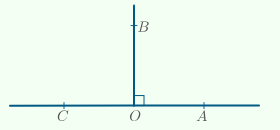
\includegraphics[width=150px]{myndir/rett_horn.png}
\end{center} & Laga bakgrunnslit á mynd \\
\hline
4171 & \hypertarget{row:4171}{rétthyrndur} &  &  &  \\
\hline
4173 & \hypertarget{row:4173}{rétthyrndur þríhyrningur} & \hyperlink{row:6438}{Þríhyrningur} með eitt \hyperlink{row:4167}{rétt horn} & Eftirfarandi er mynd af rétthyrndnum þríhyrningi:

\begin{center}
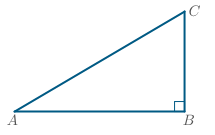
\includegraphics[width=150px]{myndir/retthyrndur_thrihyrningur.png}
\end{center} &  \\
\hline
4175 & \hypertarget{row:4175}{rétthyrningur} & \hyperlink{row:1127}{Ferhyrningur} með öll \hyperlink{row:2198}{horn} \hyperlink{row:4167}{rétt} & Eftirfarandi er mynd af rétthyrningi:

\begin{center}
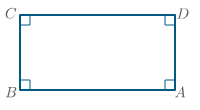
\includegraphics[width=150px]{myndir/retthyrningur.png}
\end{center} &  \\
\hline
4184 & \hypertarget{row:4184}{sívalningur, réttstæður sívalningur} & \hyperlink{row:6532}{Rúmmynd} sem afmarkast af tveimur jafnstórum \hyperlink{row:6589}{hringskífum}, sem liggja í \hyperlink{row:4509}{samsíða} \hyperlink{row:4884}{sléttum} og hafa miðjur sem liggja á \hyperlink{row:2911}{línu} sem er \hyperlink{row:6469}{hornrétt} á skífurnar, og \hyperlink{row:488}{sveigðum} \hyperlink{row:4171}{rétthyrndum} \hyperlink{row:4660}{hliðarfleti} sem fæst með því að tengja saman \hyperlink{row:4001}{punkta} \hyperlink{row:2295}{hringjanna} sem skífurnar afmarkast af með \hyperlink{row:2958}{línustriki} & Einnig er hægt að smíða sívalning með því að snúa \hyperlink{row:4175}{rétthyrningi} heilan hring um eina af \hyperlink{row:2048}{hliðum} sínum. \hyperlink{row:2860}{Lengd} hliðarinnar sem rétthyrningnum var snúið um kallast þá \textit{hæð} sívalningsins og lengd hliðanna sem eru \hyperlink{row:6469}{þverstæðar} á hana kallast \textit{geisli} sívalningsins. Sveigði flöturinn sem myndast við að rétthyrningnum er snúið kallast textit{möttull} sívalningsins. Hæð sívalnings er oft táknuð með bókstafnum $h$ og geisli hans með bókstafnum $r$. Eftirfarandi er mynd af sívalningi:

\begin{center}
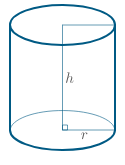
\includegraphics[width=150px]{myndir/sivalningur.png}
\end{center} & Dálítið óþjál skilgreining \\
\hline
4253 & \hypertarget{row:4253}{rót, lausn} & Ef $a$ er \hyperlink{row:981}{ekki neikvæð} \hyperlink{row:4093}{rauntala} og $n \geq 1$ er \hyperlink{row:3475}{náttúruleg tala} þá er nákvæmlega ein \hyperlink{row:2535}{jákvæð} tala $x$ sem uppfyllir $x^n = a$ sem er kölluð $n$\textit{-ta rótin} af $a$ og táknuð með $\sqrt[n]{a}$. \hyperlink{row:5397}{Talan} $a$ kallast \textit{rótarstofn} og $n$ kallast \textit{rótarvísir} & Rætur fullnægja tveimur \hyperlink{row:4150}{reiknireglum} sem oft eru kallaðar \textit{rótarreglurnar}. Þær segja:

\begin{enumerate}
    \item $\sqrt[n]{a \cdot b} = \sqrt[n]{a} \cdot \sqrt[n]{b}$
    \item $\displaystyle{\sqrt[n]{\frac{a}{b}} = \frac{\sqrt[n]{a}}{\sqrt[n]{b}}}$
\end{enumerate} & Pússa orðalag - Þarf að koma með dæmi? Minnast líka á tvinntölur? \\
\hline
4254 & \hypertarget{row:4254}{rót, núllstöð} & Fyrir \hyperlink{row:1948}{margliðu} $P$ kallast \hyperlink{row:4093}{rauntala} $r$ þannig að $P(r)=0$ \textit{rót} eða \textit{núllstöð} margliðunnar & Skilgreiningin á einnig við um margliður sem eru ekki raungildar. Sjá \hyperlink{row:1948}{margliða} &  \\
\hline
4255 & \hypertarget{row:4255}{rótarfall} & \hyperlink{row:1078}{Fall} sem varpar sérhverju \hyperlink{row:5128}{staki} $x$ úr \hyperlink{row:1343}{skilgreiningarmenginu} í $n$-tu \hyperlink{row:4253}{rót} þess $\sqrt[n]{x}$, þar sem $n \geq 2$ er \hyperlink{row:3475}{náttúruleg tala} & Ef $n$ er \hyperlink{row:2546}{slétt tala} sýnir myndin að neðan hvernig \hyperlink{row:2955}{graf} rótarfallsins \[ g_s: [0, \infty[ \to [0, \infty[; \quad g_s(x) = \sqrt[n]{x} \] lítur út. Eins og grafið endurspeglar er $g_s$ \hyperlink{row:5250}{stranglega vaxandi} og \hyperlink{row:1586}{gagntækt} og þar með \hyperlink{row:274}{andhverfanlegt}. Andhverfa þess er \hyperlink{row:927}{einskorðun} $n$-ta \hyperlink{row:6009}{veldisfallsins} við \hyperlink{row:457}{bilið} $[0, \infty[$, þ.e. \[ f_s|_{[0,\infty[}: [0, \infty[ \to [0, \infty[; \quad f_s|_{[0,\infty[}(x) = x^n \] 

\begin{center}
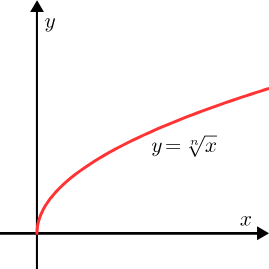
\includegraphics[width=150px]{myndir/slett_nta_rot.png}
\end{center}

Ef $n$ er \hyperlink{row:3659}{oddatala} sýnir myndin að neðan hvernig graf rótarfallsins \[ g_o: \mathbb{R} \to \mathbb{R}; \quad g_o(x) = \sqrt[n]{x} \] lítur út. Eins og grafið endurspeglar er $g_o$ stranglega vaxandi og gagntækt og því andhverfanlegt. Andhverfa þess er $n$-ta veldisfallið \[ f_o: \mathbb{R} \to \mathbb{R}; \quad f_o(x) = x^n \]

\begin{center}
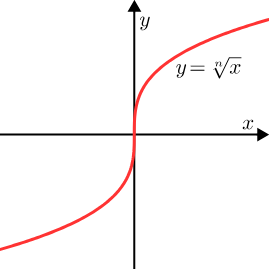
\includegraphics[width=150px]{myndir/odda_nta_rot.png}
\end{center} &  \\
\hline
4266 & \hypertarget{row:4266}{rúm} &  &  &  \\
\hline
4271 & \hypertarget{row:4271}{rúmfræði} &  &  &  \\
\hline
4294 & \hypertarget{row:4294}{Russell-þversögn} &  &  &  \\
\hline
4308 & \hypertarget{row:4308}{safn, samsafn, mengi} &  &  &  \\
\hline
4343 & \hypertarget{row:4343}{samfeldi, sameiginlegt margfeldi} & \hyperlink{row:3475}{Náttúruleg tala} $n$ kallast \textit{samfeldi} tveggja \hyperlink{row:1896}{heiltalna} ef þær \hyperlink{row:1599}{ganga báðar upp í} $n$ &  & Finna dæmi \\
\hline
4359 & \hypertarget{row:4359}{samfellt fall} &  &  &  \\
\hline
4458 & \hypertarget{row:4458}{samliggjandi, í röð} &  &  &  \\
\hline
4464 & \hypertarget{row:4464}{sammengi} & \textit{Sammengi} tveggja \hyperlink{row:3270}{mengja} $A$ og $B$ er mengi þeirra \hyperlink{row:5128}{staka} sem eru að minnsta kosti í öðru þeirra. Þetta mengi er táknað með $A \cup B$ (lesið: $A$ sam $B$) og það má rita á forminu \[ A \cup B = \{x \mid x \in A \text{ eða } x \in B\}. \] & Á \hyperlink{row:6050}{Venn-myndinni} hér að neðan er $A \cup B$ litað rautt:

\begin{center}
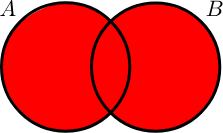
\includegraphics[width=150px]{myndir/sammengi.png}
\end{center}

Til að einfalda rithátt er sammengi $n$ mengja $A_1 \cup A_2 \cup \cdots \cup A_n$ oft ritað á forminu $\bigcup_{i=1}^n A_i$.

Sammengi eru \hyperlink{row:5472}{tengin} og \hyperlink{row:6228}{víxlin}, þ.e. fyrir öll mengi $A$, $B$ og $C$ gildir að \[ (A \cup B) \cup C = A \cup (B \cup C) \quad \text{og} \quad A \cup B = B \cup A. \] Jafnframt eru sammengi \hyperlink{row:722}{dreifin} yfir \hyperlink{row:4928}{sniðmengi}, þ.e. fyrir öll mengi $A$, $B$ og $C$ gildir að \[ A \cup (B \cap C) = (A \cup B) \cap (A \cup C) \quad \text{og} \quad (B \cap C) \cup A = (B \cup A) \cap (C \cup A). \] Loks gildir fyrir öll mengi $A$ að $A \cup \varnothing = A$ og $A \cup A = A$ &  \\
\hline
4498 & \hypertarget{row:4498}{samsemdarvörpun} & \hyperlink{row:3282}{Vörpunin} frá \hyperlink{row:3270}{mengi} $X$ yfir í $X$ sem varpar sérhverju \hyperlink{row:5128}{staki} úr $X$ í sjálft sig kallast \textit{samsemdarvörpun} mengisins $X$ og er táknuð með $\mathrm{id}_X$ &  &  \\
\hline
4509 & \hypertarget{row:4509}{samsíða, samhliða} &  &  &  \\
\hline
4514 & \hypertarget{row:4514}{samsíðungur} & \hyperlink{row:1127}{Ferhyrningur} þar sem sérhver \hyperlink{row:2048}{hlið} er \hyperlink{row:4509}{samsíða} \hyperlink{row:3396}{mótlægri hlið} sinni & Eftirfarandi er mynd af samsíðungi:

\begin{center}
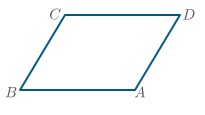
\includegraphics[width=150px]{myndir/samsidungur.png}
\end{center} &  \\
\hline
4518 & \hypertarget{row:4518}{samskeyting} & Fyrir \hyperlink{row:3282}{varpanir} $f: X \to Y$ og $g: Y \to Z$ kallast vörpunin $g \circ f: X \to Z$ sem skilgreind er með forskriftinni $(g \circ f)(x) = g(f(x))$ \textit{samskeyting} varpananna $f$ og $g$ & \hyperlink{row:6050}{Venn-myndin} að neðan sýnir varpanir $f: X \to Y$ og $g: Y \to Z$ og samskeytingu þeirra $g \circ f: X \to Z$:

\begin{center}
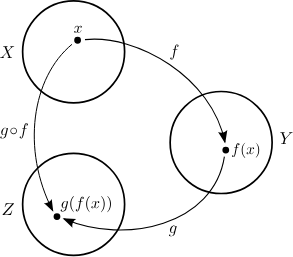
\includegraphics[width=150px]{myndir/samskeyting.png}
\end{center} &  \\
\hline
4541 & \hypertarget{row:4541}{samsvörun} & \hyperlink{row:5705}{Tvístæð vensl} milli tveggja \hyperlink{row:3270}{mengja} þar sem sérhvert \hyperlink{row:5128}{stak} í öðru hvoru menginu er venslað við nákvæmlega eitt stak í hinu menginu & Ef við lítum á \hyperlink{row:3282}{vörpun} milli mengja $X$ og $Y$ sem vensl þá jafngildir samsvörun milli $X$ og $Y$ \hyperlink{row:1586}{gagntækri vörpun} & Finna mynd? \\
\hline
4554 & \hypertarget{row:4554}{sanna} &  &  &  \\
\hline
4560 & \hypertarget{row:4560}{sanngildi} & Í \hyperlink{row:4642}{sígildri rökfræði} er sérhver \hyperlink{row:1515}{yrðing} annaðhvort \textit{sönn} eða \textit{ósönn} en kallast það \textit{sanngildi} yrðingarinnar & Sanngildi eru ýmist táknuð með $1,T$ eða $\top$ þegar um sannar yrðingar er að ræða en annars $0,F$ eða $\bot$ &  \\
\hline
4621 & \hypertarget{row:4621}{setning, meginsetning, höfuðsetning} &  &  &  \\
\hline
4624 & \hypertarget{row:4624}{setningin um ytra horn} & \hyperlink{row:4621}{Setning} í \hyperlink{row:1030}{Evklíðskri rúmfræði} sem segir að \hyperlink{row:6295}{ytra horn} \hyperlink{row:6438}{þríhyrnings} sé jafn \hyperlink{row:2223}{stórt} og samanlögð fjarlægari innri horn & Látum $ABC$ vera þríhyrning þar sem $\angle BAC$ er $35^\circ$ og $\angle ACB$ er $30^\circ$. Bæði \hyperlink{row:1677}{grannhorn} $\angle CBA$ eru þá $35^\circ + 30^\circ = 65^\circ$ samkvæmt setningunni um ytra horn & Smíða mynd af þessu dæmi \\
\hline
4625 & \hypertarget{row:4625}{sexflötungur} & \hyperlink{row:3133}{Margflötungur} með sex \hyperlink{row:1325}{hliðar} &  &  \\
\hline
4628 & \hypertarget{row:4628}{sexhyrningur} &  &  &  \\
\hline
4630 & \hypertarget{row:4630}{sextándakerfi} & ... &  &  \\
\hline
4642 & \hypertarget{row:4642}{sígild rökfræði} &  &  &  \\
\hline
4647 & \hypertarget{row:4647}{sínus} & Fyrir \hyperlink{row:4173}{rétthyrndan þríhyrning} $ABC$ þar sem $C$ er \hyperlink{row:4167}{rétt horn} er \hyperlink{row:2202}{hornafallið} \textit{sínus} af \hyperlink{row:2198}{horninu} $A$, táknað $\sin(A)$, skilgreint sem \hyperlink{row:2072}{hlutfallið} milli \hyperlink{row:2860}{lengd} \hyperlink{row:3396}{mótlægrar} \hyperlink{row:4725}{skammhliðar} og lengd \hyperlink{row:2789}{langhliðar}. Sjá eftirfarandi mynd: 

\begin{center}
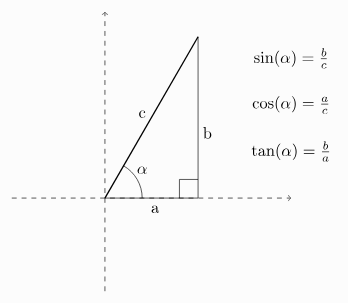
\includegraphics[width=150px]{myndir/hornafoll.png}
\end{center} & Eftirfarandi mynd sýnir hluta \hyperlink{row:2955}{grafs} sínusarfallsins: 

\begin{center}
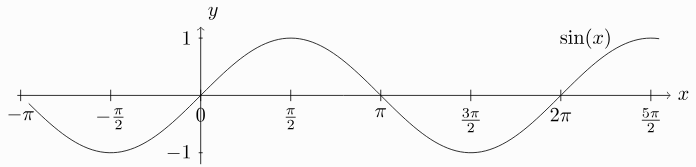
\includegraphics[width=150px]{myndir/sin.png}
\end{center} & Laga nöfn? Laga bakgrunnslit \\
\hline
4649 & \hypertarget{row:4649}{sínusregla} & Um \hyperlink{row:6438}{þríhyrning} $\Delta ABC$ gildir \textit{sínusreglan} $$ \frac{\sin(A)}{a}=\frac{\sin(B)}{b}= \frac{\sin(C)}{c}. $$ Með öðrum orðum er \hyperlink{row:2072}{hlutfallið} \hyperlink{row:3332}{milli} \hyperlink{row:4647}{sínusar} af \hyperlink{row:2198}{horni} þríhyrnings og \hyperlink{row:3396}{mótlægrar hliðar} hornsins það sama fyrir öll hornin. Þetta hlutfall er einnig jafnt $\frac{1}{2 R}$ þar sem $R$ er \hyperlink{row:2295}{geisli} \hyperlink{row:5784}{umritaðs hrings} þríhyrningsins. &  & Finna mynd til þess að taka dæmi? \\
\hline
4660 & \hypertarget{row:4660}{sívalningsflötur} & \hyperlink{row:3279}{Faldmengi} $\mathcal{C} \times I$ þar sem $\mathcal{C} \in \mathbb{R}^2$ er \hyperlink{row:1131}{ferill} og $I \subseteq \mathbb{R}$ &  & Þarf eitthvað að útskýra þetta nánar? Ég held að mynd sé ábyggilega ekki svo gagnleg \\
\hline
4725 & \hypertarget{row:4725}{skammhlið} & \hyperlink{row:2048}{Hlið} \hyperlink{row:4173}{rétthyrnds þríhyrnings} sem er ekki \hyperlink{row:2789}{langhliðin} & Á eftirfarandi mynd eru $AB$ og $BC$ skammhliðar þríhyrningsins:

\begin{center}
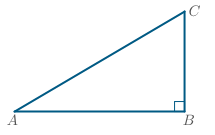
\includegraphics[width=150px]{myndir/retthyrndur_thrihyrningur.png}
\end{center} &  \\
\hline
4743 & \hypertarget{row:4743}{skauthnit, pólhnit} & \hyperlink{row:2145}{Hnitakerfi} á \hyperlink{row:1031}{evklíðska sléttu} þar sem \hyperlink{row:4001}{punktar} eru staðsettir með því að tilgreina \hyperlink{row:1204}{fjarlægð} þeirra og \hyperlink{row:5135}{stefnu} séð frá gefnum punkti $O$ sem er kallaður \textit{skaut} eða \textit{póll} & Eftirfarandi mynd sýnir hvernig hægt er að tilgreina staðsetningu punkts í \hyperlink{row:2554}{karteskum hnitum} annars vegar og pólhnitum annars vegar:

\begin{center}
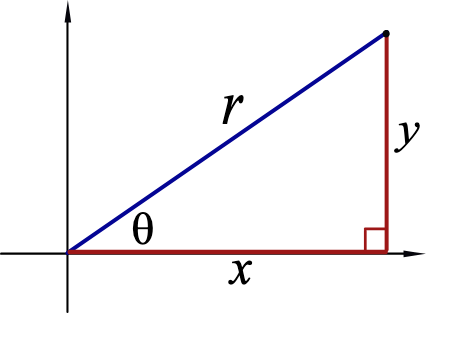
\includegraphics[width=150px]{myndir/polhnit.png}
\end{center}

Látum $O=(0,0)$ vera \hyperlink{row:5839}{upphafspunkt} karteska hnitakerfisins og $E=(1,0)$ vera einingarpunktinn á $x$-ásnum. Ef $P=(x,y)$ er punktur í sléttunni, þá mælir $r=|OP|=\sqrt{x^2+y^2}$ fjarlægð $P$ frá $O$. Stefnu $P$ séð frá $O$ má tilgreina með \hyperlink{row:483}{bogamáli} hornsins $\angle EOP$, sem við köllum \textit{stefnuhorn} punktsins $P$. Ef $P$ liggur ekki á neikvæða $x$-ásnum, þá liggur stefnuhornið á \hyperlink{row:457}{bilinu} $\left]-\pi,\pi\right[$ og það er gefið með $\arccos\left(x/\sqrt{x^2+y^2}\right)$ ef $y \geq 0$ en annars með $\arccos\left(x/\sqrt{x^2+y^2}\right)$.

Skauthnit punktsins $P=(x,y)$ eru því gefin með \hyperlink{row:5627}{tvenndinni} $(r,\theta)$.

Ekki er hægt að útvíkka skilgreininguna á stefnuhorni með skynsamlegum hætti fyrir punkta á neikvæða $x$-ásnum eða skautpunktinn $O$. Hinsvegar má snúa hnitakerfinu, og undanskilja í staðinn einhvera aðra hálflínu út frá $O$. Þannig mætti til dæmis láta stefnuhornið vera á bilinu $\left]-\pi/2,3\pi/2\right[$ og undanskilja í staðinn neikvæða hluta $y$-ássins.

Ef punktur hefur skauthnit $(r,\theta)$, þá eru kartesk hnit hans gefin með \[ x=r\,\cos\,\theta\qquad\text{og}\qquad y=r\,\sin\,\theta \] &  \\
\hline
4771 & \hypertarget{row:4771}{skerast, sníðast, skarast} & Ef \hyperlink{row:4928}{sniðmengi} tveggja \hyperlink{row:4001}{punkta}\hyperlink{row:3270}{mengja} er ekki \hyperlink{row:5564}{tómt} er sagt að mengin \textit{skerist} &  &  \\
\hline
4797 & \hypertarget{row:4797}{skilyrði} & Sjá \hyperlink{row:2836}{leiðingu} &  &  \\
\hline
4814 & \hypertarget{row:4814}{skipta í þríhyrninga} &  &  &  \\
\hline
4845 & \hypertarget{row:4845}{skurðpunktur, sniðpunktur} & \hyperlink{row:4001}{Punktur} þar sem tvö \hyperlink{row:3270}{mengi} \hyperlink{row:4771}{skerast} & Á eftirfarandi mynd skerast \hyperlink{row:2911}{línurnar} $l$ og $m$ í punktinum $A$: 

\begin{center}
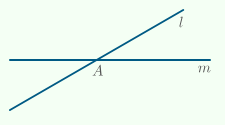
\includegraphics[width=150px]{myndir/skurdpunktur.png}
\end{center} & Laga bakgrunnslit á myndinni \\
\hline
4884 & \hypertarget{row:4884}{slétta, sléttur flötur, plan} &  &  &  \\
\hline
4891 & \hypertarget{row:4891}{sléttumynd, flatarmynd} &  &  &  \\
\hline
4904 & \hypertarget{row:4904}{sneið, kúlusneið, kúlukollur} & ... &  &  \\
\hline
4912 & \hypertarget{row:4912}{snertill, snertilína} & \hyperlink{row:2911}{Lína} sem sker \hyperlink{row:2295}{hring} í nákvæmlega einum \hyperlink{row:4001}{punkti} & Á eftirfarandi mynd má sjá hring með miðju $M$ og snertil sem liggur í gegnum punktinn $C$:

\begin{center}
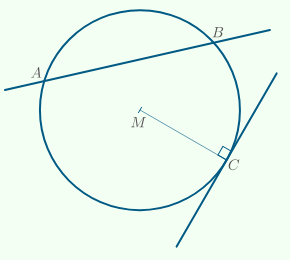
\includegraphics[width=150px]{myndir/snidill_snertill.png}
\end{center} & Minnast á að snertillinn sé hornréttur á geislann? - Laga bakgrunnslit á myndinni \\
\hline
4928 & \hypertarget{row:4928}{snið, sniðmengi, skurðmengi, skarmengi} & \textit{Sniðmengi} tveggja \hyperlink{row:3270}{mengja} $A$ og $B$ er mengi þeirra \hyperlink{row:5128}{staka} sem eru í báðum þeirra. Þetta mengi er táknað með $A \cap B$ (lesið: $A$ snið $B$) og það má rita á forminu \[ A \cap B = \{x \mid x \in A \text{ og } x \in B\}. \] & Á \hyperlink{row:6050}{Venn-myndinni} hér að neðan er $A \cap B$ litað rautt. Til að einfalda rithátt er sniðmengi $n$ mengja $A_1 \cap A_2 \cap \cdots \cap A_n$ oft ritað á forminu $\bigcap_{i=1}^n A_i$.

\begin{center}
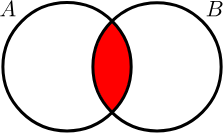
\includegraphics[width=150px]{myndir/snid.png}
\end{center}

Sniðmengi eru \hyperlink{row:5472}{tengin} og \hyperlink{row:6228}{víxlin}, þ.e. fyrir öll mengi $A$, $B$ og $C$ gildir að \[ (A \cap B) \cap C = A \cap (B \cap C) \quad \text{og} \quad A \cap B = B \cap A. \] Jafnframt eru sniðmengi \hyperlink{row:722}{dreifin} yfir \hyperlink{row:4464}{sammengi}, þ.e. fyrir öll mengi $A$, $B$ og $C$ gildir að \[ A \cap (B \cup C) = (A \cap B) \cup (A \cap C) \quad \text{og} \quad (B \cup C) \cap A = (B \cap A) \cup (C \cap A). \] Loks gildir fyrir öll mengi $A$ að $A \cap \varnothing = \varnothing$ og $A \cap A = A$ &  \\
\hline
4929 & \hypertarget{row:4929}{sniðill} & \hyperlink{row:2911}{Lína} sem sker \hyperlink{row:2295}{hring} í tveimur ólíkum \hyperlink{row:4001}{punktum} & Á eftirfarandi mynd má sjá hring með miðju $M$ og sniðil sem liggur í gegnum punktana $A$ og $B$:

\begin{center}
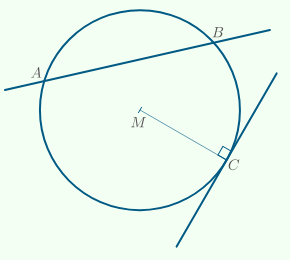
\includegraphics[width=150px]{myndir/snidill_snertill.png}
\end{center}

Ekki skal rugla saman sniðli og \hyperlink{row:5261}{streng} en munurinn er sá að sniðill er lína og strengur er \hyperlink{row:2958}{línustrik}. Sérhver strengur hrings er innihaldinn í sniðli & Laga bakgrunnslit á myndinni \\
\hline
4939 & \hypertarget{row:4939}{keila, snúðkeila, hringkeila} & \hyperlink{row:6532}{Rúmmynd} sem afmarkast af \hyperlink{row:6589}{hringskífu} og \hyperlink{row:2579}{fletinum} sem fæst með því að draga \hyperlink{row:2958}{línustrik} milli \hyperlink{row:4001}{punkta} \hyperlink{row:2295}{hringsins} sem skífan afmarkast af og eins punkts sem liggur á \hyperlink{row:2911}{línu} sem er \hyperlink{row:6469}{hornrétt} á skífuna og fer í gegnum miðju hennar & Einnig er hægt að smíða keila með því að snúa \hyperlink{row:4173}{rétthyrndum þríhyrningi} heilan hring um aðra af \hyperlink{row:4725}{skammhliðum} sínum. \hyperlink{row:2860}{Lengd} skammhliðarinnar sem þríhyrningnum var snúið um kallast þá \textit{hæð} keilunnar og lengd hinnar skammhliðarinnar kallast \textit{geisli} hennar. Sveigði flöturinn sem \hyperlink{row:2789}{langhliðin} myndar kallast \textit{möttull} keilunnar. Hæð keilu er oft táknuð með bókstafnum $h$ og geisli hennar með bókstafnum $r$. Eftirfarandi er mynd af keilu:

\begin{center}
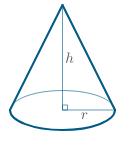
\includegraphics[width=150px]{myndir/keila.png}
\end{center} & Þarf punkturinn að liggja fyrir utan grunnflötinn? - Rosalega óþjál skilgreining \\
\hline
4954 & \hypertarget{row:4954}{snúningur} & Ef $\rho$ er \hyperlink{row:5779}{færsla} á tiltekinni \hyperlink{row:4884}{sléttu} og $M$ er \hyperlink{row:4001}{punktur} í sléttunni þá kallast $\rho$ \textit{snúningur} með \hyperlink{row:3304}{miðju} í punktinum $M$ ef hún hefur eftirfarandi eiginleika:

\begin{enumerate}
\item punktarnir $A$ og $\rho(A)$ eru í sömu \hyperlink{row:1204}{fjarlægð} frá $M$ fyrir alla punkta $A$ í sléttunni,

\item \hyperlink{row:2198}{hornin} $\angle AM\rho(A)$ eru jafn stór fyrir alla punkta $A\neq M$.
\end{enumerate} &  & Finna mynd \\
\hline
4964 & \hypertarget{row:4964}{sönnun} &  &  &  \\
\hline
4986 & \hypertarget{row:4986}{speglun} &  &  &  \\
\hline
5002 & \hypertarget{row:5002}{sporbaugur} & \hyperlink{row:3270}{Mengi} \hyperlink{row:4001}{punkta} sem uppfylla jöfnu af taginu \[ \left(\frac{x}{a}\right)^2 + \left(\frac{y}{b}\right)^2 = 1\] &  & Er til gegnsærri skilgreining? Finna mynd \\
\hline
5072 & \hypertarget{row:5072}{staðhæfing} &  &  &  \\
\hline
5097 & \hypertarget{row:5097}{stæða, stærðtákn} &  &  &  \\
\hline
5102 & \hypertarget{row:5102}{stærð} &  &  &  \\
\hline
5107 & \hypertarget{row:5107}{stærðfræði} &  &  &  \\
\hline
5114 & \hypertarget{row:5114}{stærðfræðilegur hlutur} &  &  &  \\
\hline
5117 & \hypertarget{row:5117}{stærðfræðingur} & Einstaklingur sem iðkar \hyperlink{row:5107}{stærðfræði} &  &  \\
\hline
5128 & \hypertarget{row:5128}{stak, íbúi} &  &  &  \\
\hline
5135 & \hypertarget{row:5135}{stefna, átt} &  &  &  \\
\hline
5145 & \hypertarget{row:5145}{stefnuhorn} &  &  &  \\
\hline
5161 & \hypertarget{row:5161}{stig} & Sjá \hyperlink{row:1948}{margliða} & Stig \hyperlink{row:3563}{núllmargliðunnar} er ekki unnt að skilgreina með skynsamlegum hætti sem \hyperlink{row:1896}{heila tölu} og er því stig hennar sagt vera óskilgreint &  \\
\hline
5215 & \hypertarget{row:5215}{stöðluð margliða} & \hyperlink{row:1948}{Margliða} þar sem gildi forystustuðulsins er 1 & Margliðan $x^2 + 2 x + 3$ er stöðluð margliða af stigi 2 &  \\
\hline
5227 & \hypertarget{row:5227}{stofnbrot} & \hyperlink{row:4039}{Ræð tala} skrifuð sem \hyperlink{row:234}{almennt brot} þar sem \hyperlink{row:5462}{teljarinn} er 1 og \hyperlink{row:3497}{nefnarinn} er \hyperlink{row:2535}{jákvæð} \hyperlink{row:1896}{heiltala} &  &  \\
\hline
5250 & \hypertarget{row:5250}{strangvaxandi, stranglega vaxandi, strangstígandi, stranglega stígandi, stranghækkandi, stranglega hækkandi, sívaxandi, sístígandi, síhækkandi} &  &  &  \\
\hline
5261 & \hypertarget{row:5261}{strengur} & \hyperlink{row:2958}{Línustrik} sem hefur báða endapunkta sína á \hyperlink{row:2295}{hring} kallast \textit{strengur} í hringnum & Ef miðja hringsins liggur á streng kallast sá strengur \textit{miðstrengur}. Á eftirfarandi mynd má sjá hring með miðju $M$:

\begin{center}
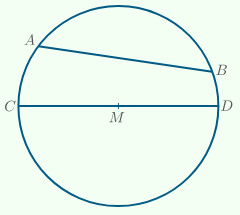
\includegraphics[width=150px]{myndir/strengur.png}
\end{center}

Strikið $AB$ er strengur í hringnum og strikið $CD$ er miðstrengur & Laga bakgrunnslit á myndinni \\
\hline
5265 & \hypertarget{row:5265}{stríkkun} & Ef $\lambda$ er \hyperlink{row:5779}{færsla} á tiltekinni \hyperlink{row:4884}{sléttu}, $k$ er \hyperlink{row:4093}{rauntala} og $M$ er \hyperlink{row:4001}{punktur} í sléttunni þá kallast $\lambda$ \textit{stríkkun} með \hyperlink{row:3304}{miðju} í punktinum $M$ ef fyrir alla punkta $P$ í sléttunni gildi að \hyperlink{row:2072}{hlutfallið} milli \hyperlink{row:2860}{lengd} \hyperlink{row:2958}{strikanna} $MP$ og $M\lambda(P)$ sé $k$, sem kallast þá \textit{kvarði} stríkkunarinnar &  & Finna mynd \\
\hline
5286 & \hypertarget{row:5286}{strýta, píramíti} & ... &  &  \\
\hline
5320 & \hypertarget{row:5320}{summa, samtala} &  &  &  \\
\hline
5325 & \hypertarget{row:5325}{sundurlæg skipting} &  &  &  \\
\hline
5329 & \hypertarget{row:5329}{sundurlægur, óskaraður} & Tvö \hyperlink{row:3270}{mengi|/ref> $X$ og $Y$ eru sögð vera \textit{sundurlæg} ef þau hafa ekkert sameiginlegt }\hyperlink{row:5128}{stak}, þ.e. ef $X \cap Y = \varnothing$ &  & Finna mynd? Er það nauðsynlegt? \\
\hline
5335 & \hypertarget{row:5335}{svæði} &  &  &  \\
\hline
5380 & \hypertarget{row:5380}{takmarkað fall, skorðað fall} & \hyperlink{row:1078}{Fall} $f: X \to Y$ kallast \textit{takmarkað} ef til er \hyperlink{row:4093}{rauntala} $C$ þannig að $|f(x)| \leq C$ fyrir öll $x \in X$ & Það að fall sé takmarkað jafngildir því að \hyperlink{row:3417}{myndmengi} þess sé \hyperlink{row:5381}{takmarkað mengi}. Til dæmis er \hyperlink{row:4647}{sínusfallið} $\sin : \mathbb{R} \to \mathbb{R}$ takmarkað vegna þess að $\sin(\mathbb{R})=[-1,1]$ sem er takmarkað mengi &  \\
\hline
5381 & \hypertarget{row:5381}{takmarkað mengi, skorðað mengi} & \hyperlink{row:4093}{Rauntalna}\hyperlink{row:3270}{mengi} $A$ kallast \textit{takmarkað} ef til er rauntala $C$ þannig að $|x| \leq C$ fyrir öll $x$ úr $A$ & Skilgreiningin á líka við \hyperlink{row:5682}{tvinntalna}mengi. Almennt er sagt að \hyperlink{row:1200}{firðrúm} $(X,d)$ sé takmarkað ef til er rauntala $C$ þannig að $d(x,y) \leq C$ fyrir öll $x,y \in X$ &  \\
\hline
5386 & \hypertarget{row:5386}{takmarkaður að neðan, skorðaður að neðan} & \hyperlink{row:4093}{rauntalna}\hyperlink{row:3270}{mengi} kallast \textit{takmarkað að neðan} ef það hefur \hyperlink{row:5818}{undirtölu} & Almennt er sagt að \hyperlink{row:4009}{hlutraðað mengi} sé takmarkað að neðan ef það hefur undirstak. Til dæmis er \hyperlink{row:1840}{hálflínan} $[0, \infty)$ takmörkuð að neðan en talan 0 er sjálf undirtala &  \\
\hline
5387 & \hypertarget{row:5387}{takmarkaður að ofan, skorðaður að ofan} & \hyperlink{row:4093}{rauntalna}\hyperlink{row:3270}{mengi} kallast \textit{takmarkað að ofan} ef það hefur \hyperlink{row:6280}{yfirtölu} & Almennt er sagt að \hyperlink{row:4009}{hlutraðað mengi} sé takmarkað að ofan ef það hefur yfirstak. Til dæmis er \hyperlink{row:1840}{hálflínan} $(-\infty, 0]$ takmörkuð að ofan en talan 0 er sjálf yfirtala &  \\
\hline
5397 & \hypertarget{row:5397}{tala} &  &  &  \\
\hline
5408 & \hypertarget{row:5408}{talnafræði, talnalist} &  &  &  \\
\hline
5415 & \hypertarget{row:5415}{talnakerfi} &  &  &  \\
\hline
5416 & \hypertarget{row:5416}{talnalína, talnaás, rauntalnalína, rauntalnaás, raunás} & \hyperlink{row:2911}{Lína} með tvo aðgreinda \hyperlink{row:4001}{punkta} $O$ (\textit{núllpunktur}) og $E$ (\textit{einingarpunktur}) sem svara til \hyperlink{row:3475}{náttúrulegu talnanna} 0 og 1. \hyperlink{row:1204}{Fjarlægðin} milli þessa punkta er notuð sem \hyperlink{row:2860}{lengdareining} og \hyperlink{row:1896}{heiltölunum} er raðað á línuna þannig að \hyperlink{row:4458}{samliggjandi} tölur eru í þessari fjarlægð frá hvor annarri &  & Þarf að minnast á hvernig ræðar og óræðar tölur dreifast inn á línuna líka? Ætti frekar að skilgreina talnalínuna beint með tilliti til rauntalna og nota þá eftirfarandi mynd

\begin{center}
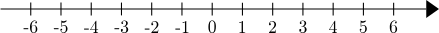
\includegraphics[width=150px]{myndir/talnalina.png}
\end{center} \\
\hline
5431 & \hypertarget{row:5431}{tangens} & Fyrir \hyperlink{row:4173}{rétthyrndan þríhyrning} $ABC$ þar sem $C$ er \hyperlink{row:4167}{rétt horn} er \hyperlink{row:2202}{hornafallið} \textit{tangens} af \hyperlink{row:2198}{horninu} $A$, táknað $\tan(A)$, skilgreint sem \hyperlink{row:2072}{hlutfallið} milli \hyperlink{row:2860}{lengd} \hyperlink{row:3396}{mótlægrar} \hyperlink{row:4725}{skammhliðar} og lengd \hyperlink{row:65}{aðlægrar} skammhliðar. Sjá eftirfarandi mynd: 

\begin{center}
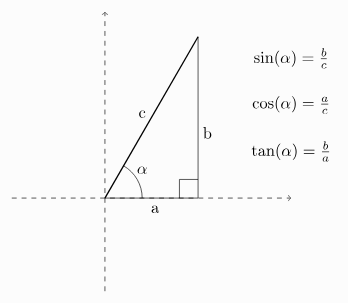
\includegraphics[width=150px]{myndir/hornafoll.png}
\end{center} & Eftirfarandi mynd sýnir hluta \hyperlink{row:2955}{grafs} tangensfallsins: 

\begin{center}
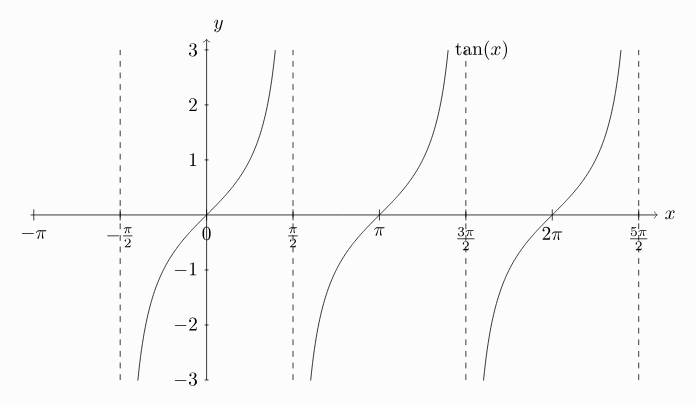
\includegraphics[width=150px]{myndir/tan.png}
\end{center} & Laga nöfn? \\
\hline
5462 & \hypertarget{row:5462}{teljari} & Sjá \hyperlink{row:234}{almennt brot} &  &  \\
\hline
5472 & \hypertarget{row:5472}{tenginn} &  &  &  \\
\hline
5473 & \hypertarget{row:5473}{tengiregla} & \hyperlink{row:5702}{Tvístæð reikniaðgerð} $\odot : X \times X \to X$ á \hyperlink{row:3270}{mengi} $X$ kallast \textit{tengin} eða að hún fullnægi \textit{tengireglunni} ef fyrir sérhver \hyperlink{row:5128}{stök} $x,y,z \in X$ gildi að $(x \odot y) \odot z = x \odot (y \odot z)$ & Margar aðgerðir í algengri notkun uppfylla tengiregluna en þó eru til ótengnar aðgerðir. Sem dæmi má nefna veldishafningu en til að mynda er $(2^3)^2 \neq 2^{(3^2)}$. Athugum að $(2^3)^2 = 8^2 = 64$ en $2^{(3^2)} = 2^9 = 512$ &  \\
\hline
5480 & \hypertarget{row:5480}{teningur, verpill, reglulegur sexflötungur} & \hyperlink{row:2559}{Kassi} þar sem allar \hyperlink{row:1325}{hliðar} eru \hyperlink{row:1163}{ferningar} & Eftirfarandi er mynd af teningi:

\begin{center}
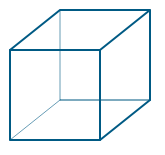
\includegraphics[width=150px]{myndir/teningur.png}
\end{center} &  \\
\hline
5486 & \hypertarget{row:5486}{tígull, tigull} & \hyperlink{row:1127}{Ferhyrningur} með allar \hyperlink{row:2048}{hliðar} jafn \hyperlink{row:2860}{langar} & Eftirfarandi er mynd af tígli:

\begin{center}
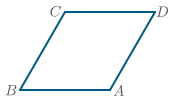
\includegraphics[width=150px]{myndir/tigull.png}
\end{center} &  \\
\hline
5558 & \hypertarget{row:5558}{tölustafur} & \hyperlink{row:5394}{Tákn} sem stendur fyrir ákveðna \hyperlink{row:3475}{náttúrulega tölu} & Algengustu tölustafirnir sem notaðir eru í stærðfræði eru svokallaðir arabískir tölustafir: 0, 1, 2, 3, 4, 5, 6, 7, 8 og 9 sem eru notaðir í \hyperlink{row:5415}{talnakerfum} með grunntölu minni en eða jöfn 10. Fyrir talnakerfi með stærri grunntölum er síðan yfirleitt sótt tákn úr rómverska stafrófinu: A, B, C og svo framvegis til þess að tákna tölur stærri en 9 &  \\
\hline
5564 & \hypertarget{row:5564}{tómt mengi, tómamengi} & \hyperlink{row:3270}{Mengið} með engin \hyperlink{row:5128}{stök}, ýmist táknað með $\emptyset, \varnothing$ eða $\{\}$ &  &  \\
\hline
5567 & \hypertarget{row:5567}{topphorn} & ... &  &  \\
\hline
5568 & \hypertarget{row:5568}{topphorn, gagnstæð horn} & \hyperlink{row:2198}{Hornið} sem \hyperlink{row:3400}{gagnstæðar} \hyperlink{row:1840}{hálflínur} við \hyperlink{row:334}{arma} \hyperlink{row:2198}{horns} mynda kallast \textit{mótlægt horn} upphaflega hornsins og sagt er að þessi tvö horn séu \textit{gagnstæð horn} & Eftirfarandi er mynd sem sýnir gagnstæð horn:

\begin{center}
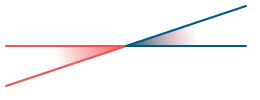
\includegraphics[width=150px]{myndir/gagnstaed_horn.png}
\end{center}

Rauðu hálflínurnar eru mótlægar við bláu hálflínurnar og rauða hornið er því mótlægt við bláa hornið. Gagnstæð horn eru alltaf jafn stór &  \\
\hline
5577 & \hypertarget{row:5577}{trapisa, hálfsamsíðungur} & \hyperlink{row:1127}{Ferhyrningur} þar sem einhver \hyperlink{row:2048}{hlið} er \hyperlink{row:4509}{samsíða} \hyperlink{row:3396}{mótlægri hlið} sinni & Eftirfarandi er mynd af trapisu:

\begin{center}
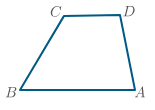
\includegraphics[width=150px]{myndir/trapisa.png}
\end{center} &  \\
\hline
5579 & \hypertarget{row:5579}{trefja} & \hyperlink{row:1366}{Frummynd} \hyperlink{row:3282}{vörpunnar} $f: X \to Y$ af \hyperlink{row:963}{einstökungnum} $\{y\}$ þar sem $y \in Y$ kallast \textit{trefja} vörpunarinnar $f$ af \hyperlink{row:5128}{stakinu}, oft táknað $f^{-1}(y)$ ef engin hætta er á misskilningi &  &  \\
\hline
5627 & \hypertarget{row:5627}{tvennd, raðtvennd, röðuð tvennd} & Par \hyperlink{row:2123}{hluta} þar sem röð skiptir máli & Fyrir tvo hluti $x \in X$ og $y \in Y$ þar sem $X$ og $Y$ eru \hyperlink{row:3270}{mengi} er tvenndin $(x,y)$ stak í \hyperlink{row:3279}{faldmenginu} $X \times Y$ &  \\
\hline
5669 & \hypertarget{row:5669}{tvílotubundinn, tvílotulegur} & Sjá skýringu við \hyperlink{row:3049}{lotubundið fall} &  & Finna mynd? \\
\hline
5673 & \hypertarget{row:5673}{tvinnfall, tvinngilt fall, tvinntölugilt fall} &  &  &  \\
\hline
5682 & \hypertarget{row:5682}{tvinntala} &  &  &  \\
\hline
5702 & \hypertarget{row:5702}{tvístæð aðgerð} & \hyperlink{row:46}{Aðgerð} á \hyperlink{row:3270}{mengi} $X$ af gerðinni $X \times X \to X$ kallast \textit{tvístæð aðgerð} & Dæmi um tvístæðar aðgerðir eru \hyperlink{row:0}{samlagning} og \hyperlink{row:3141}{margföldun} á \hyperlink{row:3270}{mengi} \hyperlink{row:4093}{rauntalna} $\mathbb{R}$ &  \\
\hline
5705 & \hypertarget{row:5705}{tvístæð vensl} &  &  &  \\
\hline
5719 & \hypertarget{row:5719}{tvíundakerfi} & ... &  &  \\
\hline
5729 & \hypertarget{row:5729}{tvívíður} &  &  &  \\
\hline
5757 & \hypertarget{row:5757}{umhverfa, andhverfa} & \textit{Andhverfa} \hyperlink{row:5128}{staks} $x$ í \hyperlink{row:3270}{mengi} $X$ með tilliti til \hyperlink{row:46}{reikniaðgerðarinnar} $\odot$ með \hyperlink{row:0}{hlutleysu} $e$ er stak $y \in X$ sem uppfyllir $x \odot y = y \odot x = e$ & Ef $\odot$ er \hyperlink{row:5473}{tengin} \hyperlink{row:3932}{ákvarðast umhverfan ótvírætt} af þessum \hyperlink{row:4797}{skilyrðum} og sérhvert stak tenginnar reikniaðgerðar hefur því í mesta lagi eina andhverfu. Athugið að andhverfa staks þarf ekki endilega að vera til. Ef reikniaðgerðin sem um ræðir er \hyperlink{row:0}{samlagning}, þá er andhverfa staksins $x$ yfirleitt táknuð með $-x$. Ef reikniaðgerðin er hins vegar \hyperlink{row:3141}{margföldun}, þá er andhverfa staksins $x$ yfirleitt táknuð með $x^{-1}$ eða $\frac1x$. & Vantar færslu fyrir samlagningu \\
\hline
5774 & \hypertarget{row:5774}{ummál} & \hyperlink{row:2860}{Lengd} \hyperlink{row:2453}{jaðar} \hyperlink{row:4891}{flatarmynds} & Ummál \hyperlink{row:6589}{hringskífu} er fengið með \hyperlink{row:363}{formúlunni} $2\pi r$ þar sem $r$ er geisli skífunnar. Ummál \hyperlink{row:3161}{marghyrnings} fæst með því að \hyperlink{row:2820}{leggja saman} allar \hyperlink{row:0}{hliðarlengdir} hans & Koma með fleiri þekktar formúlur? Er skilgreiningin of torskilin? \\
\hline
5779 & \hypertarget{row:5779}{ummyndun, myndun, færsla} & \hyperlink{row:3282}{Vörpun} $\phi : \mathbb{R}^2 \to \mathbb{R}^2$ sem uppfyllir

\begin{enumerate}
    \item punktar í tiltekinni röð á sömu línu færast á punkta í sömu röð á einhverri línu,
    \item strik sem eru jafn löng færast á strik sem eru líka jafn löng
\end{enumerate} &  & Er ekki bara verið að lýsa línulegri vörpun? \\
\hline
5784 & \hypertarget{row:5784}{umritaður hringur} & Ef \hyperlink{row:2235}{hornpunktar} \hyperlink{row:3161}{marghyrnings} liggja allir á gefnum \hyperlink{row:2295}{hring}, þá kallast hringurinn \textit{umritaður hringur} marghyrningsins & Eftirfarandi mynd sýnir umritaðan hring \hyperlink{row:4628}{sexhyrnings}:

\begin{center}
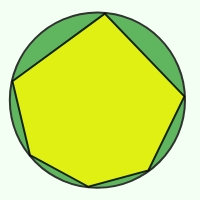
\includegraphics[width=150px]{myndir/umritadur_hringur.png}
\end{center} & Laga bakgrunnslit á myndinni \\
\hline
5818 & \hypertarget{row:5818}{undirstak, undirskorða, undirtala} & Fyrir \hyperlink{row:4093}{rauntalna}\hyperlink{row:3270}{mengi} $A$ kallast rauntalan $L$ \textit{undirtala} mengisins $A$ ef fyrir öll $x \in A$ gildir að $x \geq L$ & Almennt getur \hyperlink{row:4009}{hlutraðað mengi} hugsanlega átt sér \textit{undirstak}. Slíkt \hyperlink{row:5128}{stak} þarf hins vegar ekki endilega að vera til, sem dæmi á mengi rauntalna $\mathbb{R}$ sér ekkert undirstak &  \\
\hline
5822 & \hypertarget{row:5822}{undirstöðusetning algebrunnar, grunnsetning algebrunnar} & \textit{Undirstöðusetning algebrunnar} segir að sérhver \hyperlink{row:1948}{margliða} yfir \hyperlink{row:5682}{tvinntölurnar} $\mathbb{C}$ með stig $\geq 1$ eigi sér \hyperlink{row:4254}{núllstöð} í $\mathbb{C}$ & Þar sem tvinntala $r$ er núllstöð í margliðu $P$ yfir $\mathbb{C}$ þá og því aðeins að margliðan $(x - r)$ gangi upp í $P$, þá gefur undirstöðusetningin að sérhverja margliðu $P$ yfir $\mathbb{C}$ megi skrifa á eftirfarandi formi:

\[P = (x - r_{1})^{a_{1}} (x - r_{2})^{a_{2}} \cdots (x - r_{k})^{a_{k}}\]

þar sem $r_{1},\ldots,r_{k}$ eru allar núllstöðvar $P$ í $\mathbb{C}$ og $a_{1},\ldots,a_{k}$ kallast \textit{margfeldni} þeirra. Að rita margliðuna á þessu formi kallast að \textit{frumþátta} hana yfir $\mathbb{C}$. Yfir \hyperlink{row:4093}{rauntölurnar} tekur undirstöðusetningin eftirfarandi form:

\textit{Ef $P$ er \hyperlink{row:5215}{stöðluð margliða} yfir $\mathbb{R}$, þá má skrifa $P$ sem margfeldi af fyrsta stigs margliðum $(x-r_i)$ og \hyperlink{row:316}{annars stigs margliðum} $x^2+ax+b$ sem hafa enga núllstöð yfir $\mathbb{R}$. Tölurnar $r_i$ eru allar núllstöðvar margliðunnar} & Vantar færslu fyrir fyrsta stigs margliðu? \\
\hline
5824 & \hypertarget{row:5824}{undirstöðusetning reikningslistarinnar, grunnsetning reikningslistarinnar, frumþáttunarsetning} & \textit{Undirstöðusetning reikningslistarinnar} segir að sérhverja \hyperlink{row:3475}{náttúrulega tölu} $n$ megi skrifa á nákvæmlega einn hátt sem \hyperlink{row:3118}{margfeldi} af \hyperlink{row:1468}{frumtölum}. Nánar tiltekið gildir fyrir sérhverja náttúrulega tölu $n$ að til eru \hyperlink{row:3932}{ótvírætt ákvarðaðar} frumtölur $p_{1}, \ldots ,p_{k}$ og náttúrulegar tölur $a_{1}, \ldots ,a_{k}$ þannig að:

\[ n = {p_{1}}^{a_{1}} \cdot {p_{2}}^{a_{2}} \cdot \ldots \cdot {p_{k-1}}^{a_{k-1}} \cdot {p_{k}}^{a_{k}} \] 

þar sem $p_{i} < p_{j}$ þegar $i < j$. Að skrifa töluna $n$ á þessu formi kallast að \textit{frumþátta} hana. \hyperlink{row:5397}{Tölurnar} $p_{1}, \ldots, p_{k}$ kallast þá \textit{frumþættir} tölunnar $n$ og $a_{i}$ kallast \textit{margfeldni} frumþáttarins $p_{i}$ & Eftirfarandi er frumþáttun á tölunni 252:

\begin{center}
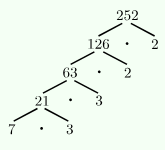
\includegraphics[width=150px]{myndir/undirstodusetning_reikningslistarinnar.png}
\end{center}

Af myndinni sést að 252 frumþáttast sem $252 = 2^2 \cdot 3^2 \cdot 7$ & Laga bakgrunnslit á myndinni \\
\hline
5839 & \hypertarget{row:5839}{upphaf, upphafspunktur, hnitmiðja, hnitamiðja} &  &  &  \\
\hline
5850 & \hypertarget{row:5850}{upphafspunktur} &  &  &  \\
\hline
5871 & \hypertarget{row:5871}{úrkynjaður} &  &  &  \\
\hline
5902 & \hypertarget{row:5902}{úthorn, fyllihorn} & ... &  &  \\
\hline
5954 & \hypertarget{row:5954}{valfrumsenda, valfrumsetning, frumsenda um val, frumsetning um val} &  &  &  \\
\hline
5963 & \hypertarget{row:5963}{varðveita, rækja} &  &  &  \\
\hline
5968 & \hypertarget{row:5968}{varpgildi} &  &  &  \\
\hline
6007 & \hypertarget{row:6007}{veldi} &  &  &  \\
\hline
6009 & \hypertarget{row:6009}{veldisfall} & \hyperlink{row:1078}{Fall} sem varpar sérhverju \hyperlink{row:5128}{staki} $x$ í $n$-ta \hyperlink{row:6007}{veldi} þess $x^n$, þar sem $n \geq 2$ er \hyperlink{row:3475}{náttúruleg tala} &  &  \\
\hline
6013 & \hypertarget{row:6013}{veldismengi} & \hyperlink{row:3270}{Mengið} sem samanstendur af öllum \hyperlink{row:2098}{hlutmengjum} í tilteknu mengi $X$, táknað með $\mathcal{P}(X)$ & Almennt gildir að ef fjöldi \hyperlink{row:5128}{staka} í mengi $X$ er $n$, þar sem $n$ er \hyperlink{row:3475}{náttúruleg tala}, er fjöldi staka í veldismengi þess $2^n$. Dæmi um veldismengi fæst með því að setja $X = \{1,2,3\}$. Hlutmengjunum í $X$ má þá skipta í fjóra hópa eftir fjölda staka:

$\varnothing$ er það hlutmengi í $X$ sem hefur ekkert stak.
$\{1\}$, $\{2\}$ og $\{3\}$ eru þau hlutmengi í $X$ sem hafa eitt stak.
$\{1,2\}$, $\{1,3\}$ og $\{2,3\}$ eru þau hlutmengi í $x$ sem hafa tvö stök.
$\{1,2,3\}$ er það hlutmengi í $X$ sem hefur þrjú stök.
Veldismengið $\mathcal{P}(X)$ er þá mengið sem samanstendur af öllum framantöldum mengjum, þ.e. \[ \mathcal{P}(X) = \{ \varnothing,\{1\},\{2\},\{3\},\{1,2\},\{1,3\},\{2,3\},\{1,2,3\} \}. \] &  \\
\hline
6050 & \hypertarget{row:6050}{Venn-mynd} & Myndræn \hyperlink{row:1416}{framsetning} á innbyrðis afstöðu ólíkra \hyperlink{row:3270}{mengja} þar sem \hyperlink{row:3016}{lokaðir ferlar} (eins og \hyperlink{row:2295}{hringir}, \hyperlink{row:5002}{sporbaugar}, \hyperlink{row:1127}{ferhyrningar} o.s.frv.) eru notaðir til að tákna mengi og \hyperlink{row:5335}{svæðið} sem er innan ferlanna táknar \hyperlink{row:5128}{stökin} í menginu & Eftirfarandi mynd er dæmi um Venn-mynd:

\begin{center}
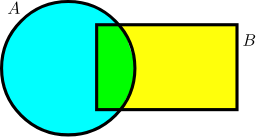
\includegraphics[width=150px]{myndir/venn.png}
\end{center}

Hringurinn táknar mengið $A$ og svæðið innan hans táknar stökin í $A$, \hyperlink{row:4175}{rétthyrningurinn} táknar mengið $B$ og svæðið innan hans táknar stökin í $B$. Bláa svæðið samanstendur af þeim stökum sem eru í $A$ en ekki í $B$ (þau eru innan hringsins en utan rétthyrningsins), gula svæðið samanstendur af þeim stökum sem eru í $B$ en ekki í $A$ (þau eru innan rétthyrningsins en utan hringsins) og græna svæðið samanstendur af þeim stökum sem eru bæði í $A$ og í $B$ (þau eru innan bæði hringsins og rétthyrningsins) &  \\
\hline
6051 & \hypertarget{row:6051}{vensl} &  &  &  \\
\hline
6087 & \hypertarget{row:6087}{vídd, víddartala, rúmvídd} &  &  &  \\
\hline
6167 & \hypertarget{row:6167}{vinstri dreifiregla} & Sjá \hyperlink{row:723}{dreifiregla} &  &  \\
\hline
6228 & \hypertarget{row:6228}{víxlinn} &  &  &  \\
\hline
6233 & \hypertarget{row:6233}{víxlregla} & \hyperlink{row:5702}{Tvístæð reikniaðgerð} $\odot : X \times X \to X$ á \hyperlink{row:3270}{mengi} $X$ kallast \textit{víxlin} eða að hún fullnægi \textit{víxlreglunni} ef fyrir sérhver \hyperlink{row:5128}{stök} $x,y \in X$ gildi að $x \odot y = y \odot x$ & Dæmi um víxlna reikniaðgerð er \hyperlink{row:3141}{margföldun} \hyperlink{row:4093}{rauntalna} en um öll $x,y \in \mathbb{R}$ gildir $xy=yx$ &  \\
\hline
6252 & \hypertarget{row:6252}{x-ás} &  &  &  \\
\hline
6253 & \hypertarget{row:6253}{y-ás} &  &  &  \\
\hline
6280 & \hypertarget{row:6280}{yfirstak, yfirskorða, yfirtala} & Fyrir \hyperlink{row:4093}{rauntalna}\hyperlink{row:3270}{mengi} $A$ kallast rauntalan $U$ \textit{yfirtala} mengisins $A$ ef fyrir öll $x \in A$ gildir að $x \leq U$ & Almennt getur \hyperlink{row:4009}{hlutraðað mengi} hugsanlega átt sér \textit{yfirstak}. Slíkt \hyperlink{row:5128}{stak} þarf hins vegar ekki endilega að vera til, sem dæmi á mengi rauntalna $\mathbb{R}$ sér ekkert yfirstak &  \\
\hline
6295 & \hypertarget{row:6295}{ytra horn, utanvert horn} & \hyperlink{row:1677}{Grannhorn} tiltekins \hyperlink{row:2198}{horns} í \hyperlink{row:3161}{marghyrningi}. Horn marghyrningsins kallast þá \textit{innri horn} & Á eftirfarandi mynd er $\angle DBC$ ytra horn við \hyperlink{row:6438}{þríhyrninginn} $ABC$ því það er grannhorn $\angle CBA$:

\begin{center}
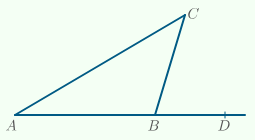
\includegraphics[width=150px]{myndir/ytrahorn.png}
\end{center} 

Hornin $\angle BAC$ og $\angle ACB$ kallast jafnframt \textit{fjarlæg innri horn} við ytra hornið $\angle DBC$ & Laga bakgrunnslit á myndinni \\
\hline
6314 & \hypertarget{row:6314}{Zermelo-Fraenkel-mengjafræði} &  &  &  \\
\hline
6315 & \hypertarget{row:6315}{Zermelo-Fraenkel-mengjafræði með valfrumsendu} &  &  &  \\
\hline
6402 & \hypertarget{row:6402}{þrepasönnun, þrepunarsönnun, rakin sönnun} & ... &  &  \\
\hline
6436 & \hypertarget{row:6436}{þríhyrningsójafna} &  &  &  \\
\hline
6438 & \hypertarget{row:6438}{þríhyrningur} & \hyperlink{row:3161}{Marghyrningur} með þrjár \hyperlink{row:2048}{hliðar} & Eftirfarandi er mynd af þríhyrningi:

\begin{center}
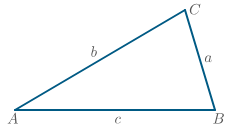
\includegraphics[width=150px]{myndir/thrihyrningur.png}
\end{center} &  \\
\hline
6454 & \hypertarget{row:6454}{þrívíður} &  &  &  \\
\hline
6469 & \hypertarget{row:6469}{þver, þverstæður, hornréttur, þverlægur} &  &  &  \\
\hline
6473 & \hypertarget{row:6473}{þverás} &  &  &  \\
\hline
6489 & \hypertarget{row:6489}{þvermál} & \hyperlink{row:2295}{Hringur} með geisla $r$ hefur \textit{þvermál} $2r$ &  &  \\
\hline
6531 & \hypertarget{row:6531}{þykkvafræði, þrívíð rúmfræði} & ... &  &  \\
\hline
6532 & \hypertarget{row:6532}{þykkvi, rúmskiki, líkami, hlutur, rúmmynd, gripur} &  &  &  \\
\hline
6589 & \hypertarget{row:6589}{hringskífa, hringflötur} & \hyperlink{row:4891}{Sléttumynd} sem afmarkast af \hyperlink{row:2295}{hring} & Eftirfarandi er mynd af hringskífu með miðju $M$ og geisla $r$. Skyggða \hyperlink{row:5335}{svæðið} tilheyrir allt hringskífunni:

\begin{center}
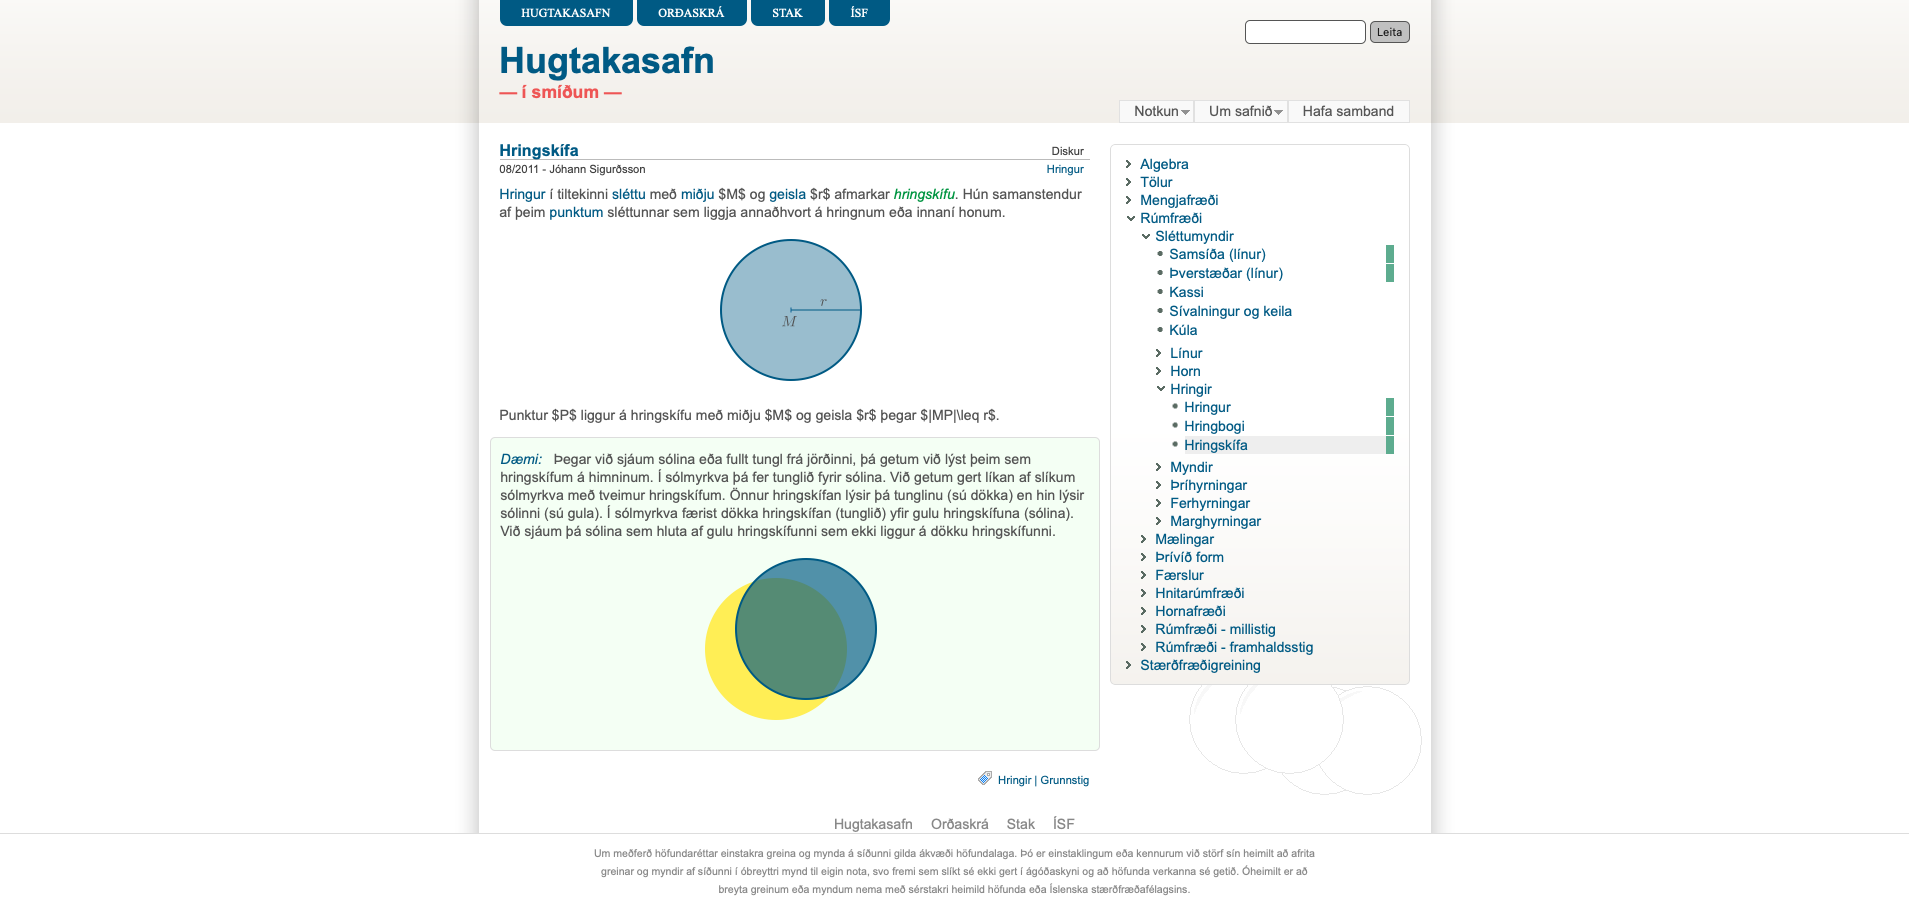
\includegraphics[width=150px]{myndir/hringskifa.png}
\end{center} &  \\
\hline
6592 & \hypertarget{row:6592}{jafngildisvensl} & \hyperlink{row:5705}{Tvístæð vensl} á \hyperlink{row:3270}{mengi} $X$ sem uppfylla eftirfarandi þrjú \hyperlink{row:4797}{skilyrði}: 

\begin{enumerate}
    \item Sérhvert \hyperlink{row:5128}{stak} í menginu er venslað við sjálft sig (\textit{spegilvirkni})
    \item Fyrir sérhver stök $x,y \in X$ gildir að ef $x$ er venslað við $y$, þá er $y$ líka venslað við $x$ (\textit{samhverfni})
    \item Fyrir sérhver stök $x,y,z \in X$ gildir að ef $x$ er venslað við $y$ og $y$ er venslað við $z$, þá er $x$ einnig venslað við $z$ (\textit{gegnvirkni})
\end{enumerate} & Jafngildisvensl á mengi $X$ eru ákveðin útvíkkun á hugtakinu að tvö \hyperlink{row:5128}{stök} úr $X$ séu \hyperlink{row:2474}{jöfn}, enda uppfylla venslin $=$ skilyrði þess að vera jafngildisvensl. Sérhver jafngildisvensl á $X$ mynda \hyperlink{row:5325}{skiptingu} á $X$ í \hyperlink{row:5329}{sundurlæga} \hyperlink{row:2489}{jafngildisflokka}. Venslin $=$ eru sértilfelli þar sem jafngildisflokkarnir eru allir \hyperlink{row:963}{einstökungar}, með öðrum orðum eru tvö stök $x,y \in X$ jöfn þá og því aðeins að þau séu sama stakið. Almenn jafngildisvensl gera manni hins vegar kleift að einblína á ákveðna \hyperlink{row:803}{eiginleika} stakanna og líta á tvö stök sem eru vensluð saman sem jafngild þó að þau séu ekki jöfn stök. Dæmi um jafngildisvensl eru venslin ``eru \hyperlink{row:4509}{samsíða}'' á mengi \hyperlink{row:2911}{lína} í \hyperlink{row:1031}{evklíðskri sléttu} en þá ákveðum við að einblína einungis á \hyperlink{row:1863}{halla} línanna og hunsum alveg hvaða \hyperlink{row:4001}{punktar} liggja á þeim &  \\
\hline
6624 & \hypertarget{row:6624}{ósannur} & Sjá \hyperlink{row:4560}{sanngildi} &  &  \\
\hline
6659 & \hypertarget{row:6659}{sannur} & Sjá \hyperlink{row:4560}{sanngildi} &  &  \\
\hline
\hline
\end{longtable}
